\documentclass[12pt, a4paper, oneside, openany,DIV=16 headings=small]{scrbook}

% Eingelagerte Präambel
% Sprach-/Font-Setup
\usepackage[T1]{fontenc}
\usepackage[utf8]{inputenc}
\usepackage[ngerman]{babel}
\usepackage{lmodern}
\usepackage{microtype}
\usepackage{csquotes}
\usepackage{changepage}
\usepackage{listings}
\usepackage{listingsutf8}

% Mathe & Physik
\usepackage{amsmath, amssymb, amsthm, tcolorbox}
\usepackage{siunitx}     % \SI{...}{...}
\sisetup{locale=DE, per-mode=symbol}
\usepackage{physics}     % \dv, \grad, \laplacian etc. (optional)

% Grafik, Tabellen
\usepackage{graphicx}
\usepackage{subcaption}
\usepackage{booktabs}
\usepackage{array}
\usepackage{tikz}
\usepackage{pgfplots}
\pgfplotsset{compat=newest}

% Referenzen/Links
\usepackage[hidelinks]{hyperref}
\usepackage[capitalise,noabbrev]{cleveref}

% Code-Listings (ohne shell-escape)
\usepackage{listings}
\lstset{
  basicstyle=\ttfamily\small,
  frame=single,
  numbers=left,
  numberstyle=\tiny,
  breaklines=true,
  tabsize=2,
  language=Python
}

% Bibliographie
\usepackage[
  backend=biber,
  style=authoryear,
  giveninits=true,
  maxcitenames=2, maxbibnames=20,
  uniquename=false, sorting=nyt,
  doi=false, isbn=false, url=false
]{biblatex}

\addbibresource{bib/references.bib}

% --- Glossar ---
%\usepackage{glossaries-extra}
%\setabbreviationstyle[acronym]{long-short}
%\makeglossaries

% Einfache, saubere Makros
\newcommand{\alphastar}{\ensuremath{\alpha^{\ast}}}
\newcommand{\ERTh}{Energie-Resonanz-Theorie}
\newcommand{\helm}{Helmholtz-Gleichung}
\newcommand{\robin}{Robin-Randbedingung}

% Vektor/Laplace etc. (falls physics nicht genutzt wird)
% \newcommand{\laplace}{\nabla^2}

% Einheiten-Kürzel
\newcommand{\GB}{\ensuremath{\,\mathrm{GB}}}
\newcommand{\EB}{\ensuremath{\,\mathrm{EB}}}

% Abstract-Umgebung für scrbook definieren
\providecommand{\abstractname}{Zusammenfassung}
\makeatletter
\newenvironment{abstract}{%
  \cleardoublepage
  \chapter*{\abstractname}%
  \addcontentsline{toc}{chapter}{\abstractname}%
  \markboth{\abstractname}{\abstractname}%
}{\par}
\makeatother

% Lockerere Float-Regeln
\makeatletter
\renewcommand{\topfraction}{0.95}      % Anteil oben: bis 95% Float erlaubt
\renewcommand{\bottomfraction}{0.95}   % Anteil unten: bis 95% Float
\renewcommand{\textfraction}{0.01}     % Mindesttextanteil auf Seite: nur 5%
\renewcommand{\floatpagefraction}{0.5}
\setcounter{topnumber}{3}              % max. Floats oben
\setcounter{bottomnumber}{2}           % max. Floats unten
\setcounter{totalnumber}{5}            % max. Floats gesamt pro Seite
\makeatother

% (optional, für engere Abstände)
\setlength{\textfloatsep}{10pt plus 2pt minus 2pt}
\setlength{\intextsep}{10pt plus 2pt minus 2pt}
\theoremstyle{definition}
\newtheorem{definition}{Definition}[chapter]
\newtheorem{annahme}{Annahme}[chapter]

\theoremstyle{plain}
\newtheorem{satz}{Satz}[chapter]
\newtheorem{folgerung}{Folgerung}[chapter]

\theoremstyle{remark}
\newtheorem{bemerkung}{Bemerkung}[chapter]


% - Benutzung im Text:
%   \gls{alpha-star}, \Gls{spiralis}, \acrshort{ERT}, \acrlong{ART} etc.

% Haupt-Begriffe

\newglossaryentry{alpha-star}{%
  name={\ensuremath{\alpha^\star}},
  sort={alpha-star},
  text={\ensuremath{\alpha^\star}},
  description={%
    Dimensionsloser Operator der Energie–Zeit–Abweichung zur idealen Periode; in der ERT der \emph{Öffnungswinkel} der realen Spiraldynamik. %
    \ensuremath{\alpha^\star} legt die aperiodische Phasenverschiebung fest und bestimmt damit Resonanz, Skalenkopplung und Wahrnehmungsrahmen.},
  plural={\ensuremath{\alpha^\star}}%
}

\newglossaryentry{spiralis}{%
  name={Spiralis},
  sort={spiralis},
  description={%
    Erweiterung der Sinusfunktion zur \emph{dreidimensionalen, aperiodischen} Felddynamik. %
    Die Spiralis erzeugt aus drei dualen Raumrichtungen ein fraktales, resonantes Feld, dessen Zeitverlauf als geometrische Folge erscheint.},
  plural={Spirales}%
}

\newglossaryentry{aperiodizitaet}{%
  name={Aperiodizität},
  sort={aperiodizitaet},
  description={%
    Abwesenheit exakter Wiederkehr. In der ERT ist Aperiodizität eine essentielle Eigenschaft realer Dynamik: %
    Umlaufbahnen, Energieflüsse und Kopplungen schließen nicht exakt, sondern nähern sich asymptotisch periodischen Mustern an.}%
}

\newglossaryentry{resonanz}{%
  name={Resonanz},
  sort={resonanz},
  description={%
    Überlagerung kohärenter Wellenanteile mit Stabilisierung bestimmter Strukturen (Knoten/Zonen). %
    In der ERT entstehen so hierarchische Kopplungen (Proton $\rightarrow$ H $\rightarrow$ H$_2$ $\rightarrow$ H$^2$O).}%
}

\newglossaryentry{helmholtz}{%
  name={Helmholtz-Gleichung},
  sort={helmholtz},
  description={%
    Partielle Differentialgleichung, die stationäre Wellenfelder beschreibt. %
    In der ERT dient sie als Ausgangspunkt für das Eigenwertproblem im dreidimensionalen Randwert-Setup.}%
}

\newglossaryentry{robin}{%
  name={Robin-Randbedingung},
  sort={robin},
  description={%
    Lineare Randbedingung der Form \ensuremath{a u + b\,\partial_n u = c} an der Grenze des Lösungsgebiets. %
    In der ERT modelliert sie Energiefluss und Balance zwischen Feld und „Außenraum“.}%
}

\newglossaryentry{eigenwert}{%
  name={Eigenwert},
  sort={eigenwert},
  description={%
    Spektralbegriffe des Randwertproblems: Eigenwerte quantisieren zulässige Feldmodi; Eigenfunktionen sind die zugehörigen räumlichen Muster. %
    Der numerische Scan/ Fit der ERT identifiziert ein konsistentes Spektralsignal für \gls{alpha-star}.}%
}

\newglossaryentry{wahrnehmungsrahmen}{%
  name={Wahrnehmungsrahmen},
  sort={wahrnehmungsrahmen},
  description={%
    Effektive, periodische Maske menschlicher Messung und Erfahrung. %
    In der ERT wird Zeit als aus dem Feld emergierende Geometrie verstanden; der Wahrnehmungsrahmen begrenzt Sichtbarkeit (z.\,B. Lichtgeschwindigkeit, EM-Spektrum).}%
}

\newglossaryentry{dualitaet}{%
  name={Dualität (Richtungen)},
  sort={dualitaet},
  description={%
    Jede Raumdimension besitzt zwei Richtungen; Negativität wird nicht benötigt. %
    Die dreifache Dualität erzeugt acht erste Überlagerungspunkte (Ecken eines Würfels) als elementare Resonanzstruktur.}%
}

\newglossaryentry{achter-raster}{%
  name={8er-Raster},
  sort={achter-raster},
  description={%
    Diskretisierung entlang der acht kubischen Richtungen. %
    Dient im ERT-Scan als minimaler symmetrischer Suchraum, in dem Resonanzknoten zuverlässig detektierbar werden.}%
}

\newglossaryentry{hierarchie}{%
  name={Diadische Hierarchie},
  sort={hierarchie},
  description={%
    Skalierung/Einbettung von Resonanzknoten über Faktoren von zwei und acht, wodurch fraktale, selbstähnliche Strukturen über Skalen hinweg entstehen.}%
}

\newglossaryentry{normalisierung}{%
  name={Normalisierung},
  sort={normalisierung},
  description={%
    Abbildung der berechneten Felder auf \([0,1]\) zur Visualisierung. %
    Der Punkt \mbox{\(0{,}5\)} markiert die Wahrnehmungsnull (Raum), während \(\,1-\alpha^\star/10\,\) die sichtbare Informationsgrenze setzt.}%
}

\newglossaryentry{em-colormap}{%
  name={EM-Colormap (ERT)},
  sort={em-colormap},
  description={%
    Farbcodierung, die das sichtbare Spektrum (Violett\,$\to$\,Weiß) in Einklang mit \gls{alpha-star} abbildet, inkl.\ UV/IR-Interpretation als „Rand“-Informationen des Wahrnehmungsfensters.}%
}

\newglossaryentry{vti}{%
  name={VTI-Volumen},
  sort={vti},
  description={%
    VTK ImageData-Dateiformat für reguläre Gitter (ParaView-kompatibel), genutzt zur Speicherung der berechneten ERT-Felder (z.\,B. Proton, H, H$_2$, O, H$^2$O).}%
}

\newglossaryentry{paraview}{%
  name={ParaView},
  sort={paraview},
  description={%
    Open-Source-Werkzeug zur Volumenvisualisierung. %
    In der ERT dient ParaView als experimentelle Bühne zur Sichtbarmachung der Spiralis-Felder und ihrer Hierarchien.}%
}

\newglossaryentry{residuum}{%
  name={Residuum/Residuen-Fit},
  sort={residuum},
  description={%
    Maß für Abweichungen zwischen Modell und Daten; in der ERT zur Verifikation von \gls{alpha-star} über Skalen (atomar, kosmologisch) eingesetzt.}%
}

\newglossaryentry{wahrnehmungsfilter}{%
  name={Wahrnehmungsfilter (UV/IR)},
  sort={wahrnehmungsfilter},
  description={%
    Reduktion der Opazität außerhalb des sichtbaren Spektrums (UV, IR), um die strukturtragenden Bereiche der Felder klar erkennbar zu machen.}%
}

\newglossaryentry{zeit-als-geometrie}{%
  name={Zeit als Geometrie},
  sort={zeit-als-geometrie},
  description={%
    ERT-Kerngedanke: Zeit ist keine unabhängige Koordinate, sondern die emergente Folge des aperiodischen Spiralverlaufs im dreidimensionalen Feld.}%
}

% ---------- Akronyme ----------

\newacronym{ERT}{ERT}{Energie-Resonanz-Theorie}
\newacronym{ART}{ART}{Allgemeine Relativitätstheorie}
\newacronym{EM}{EM}{Elektromagnetisch / Elektromagnetisches Spektrum}
\newacronym{CMB}{CMB}{Kosmische Mikrowellen-Hintergrundstrahlung}
\newacronym{VTK}{VTK}{Visualization Toolkit (Dateiformate/IO)}

%\usepackage[T1]{fontenc}
\usepackage[utf8]{inputenc}
\usepackage{lmodern}
\usepackage{amsmath,amssymb}
\usepackage{placeins}


\lstdefinestyle{ERTlisting}{
  language=Python,
  basicstyle=\ttfamily\footnotesize,
  breaklines=true,
  columns=fullflexible,
  showstringspaces=false,
  frame=single
}

\lstset{
  style=ERTlisting,
  inputencoding=utf8,
  literate=
    {ä}{{\"a}}1 {ö}{{\"o}}1 {ü}{{\"u}}1
    {Ä}{{\"A}}1 {Ö}{{\"O}}1 {Ü}{{\"U}}1
    {ß}{{\ss}}1
    {–}{{-}}1 {—}{{-}}1
}

\usepackage{graphicx}
\graphicspath{{Grafiken/}}

\begin{document}
\begin{titlepage}
    \thispagestyle{empty}
    \centering
    {\LARGE\bfseries Die Energie-Resonanz-Theorie (ERT)\par}
     \vspace{0.3cm}
    {\large Eine andere Perspektive auf Raum, Resonanz und Struktur\par} 
    \vspace{1.2cm}
    {\Large Steven Trümpert\par}
    \vspace{0.6cm}
    {\large \today\par}
    \vspace{3.0cm}
    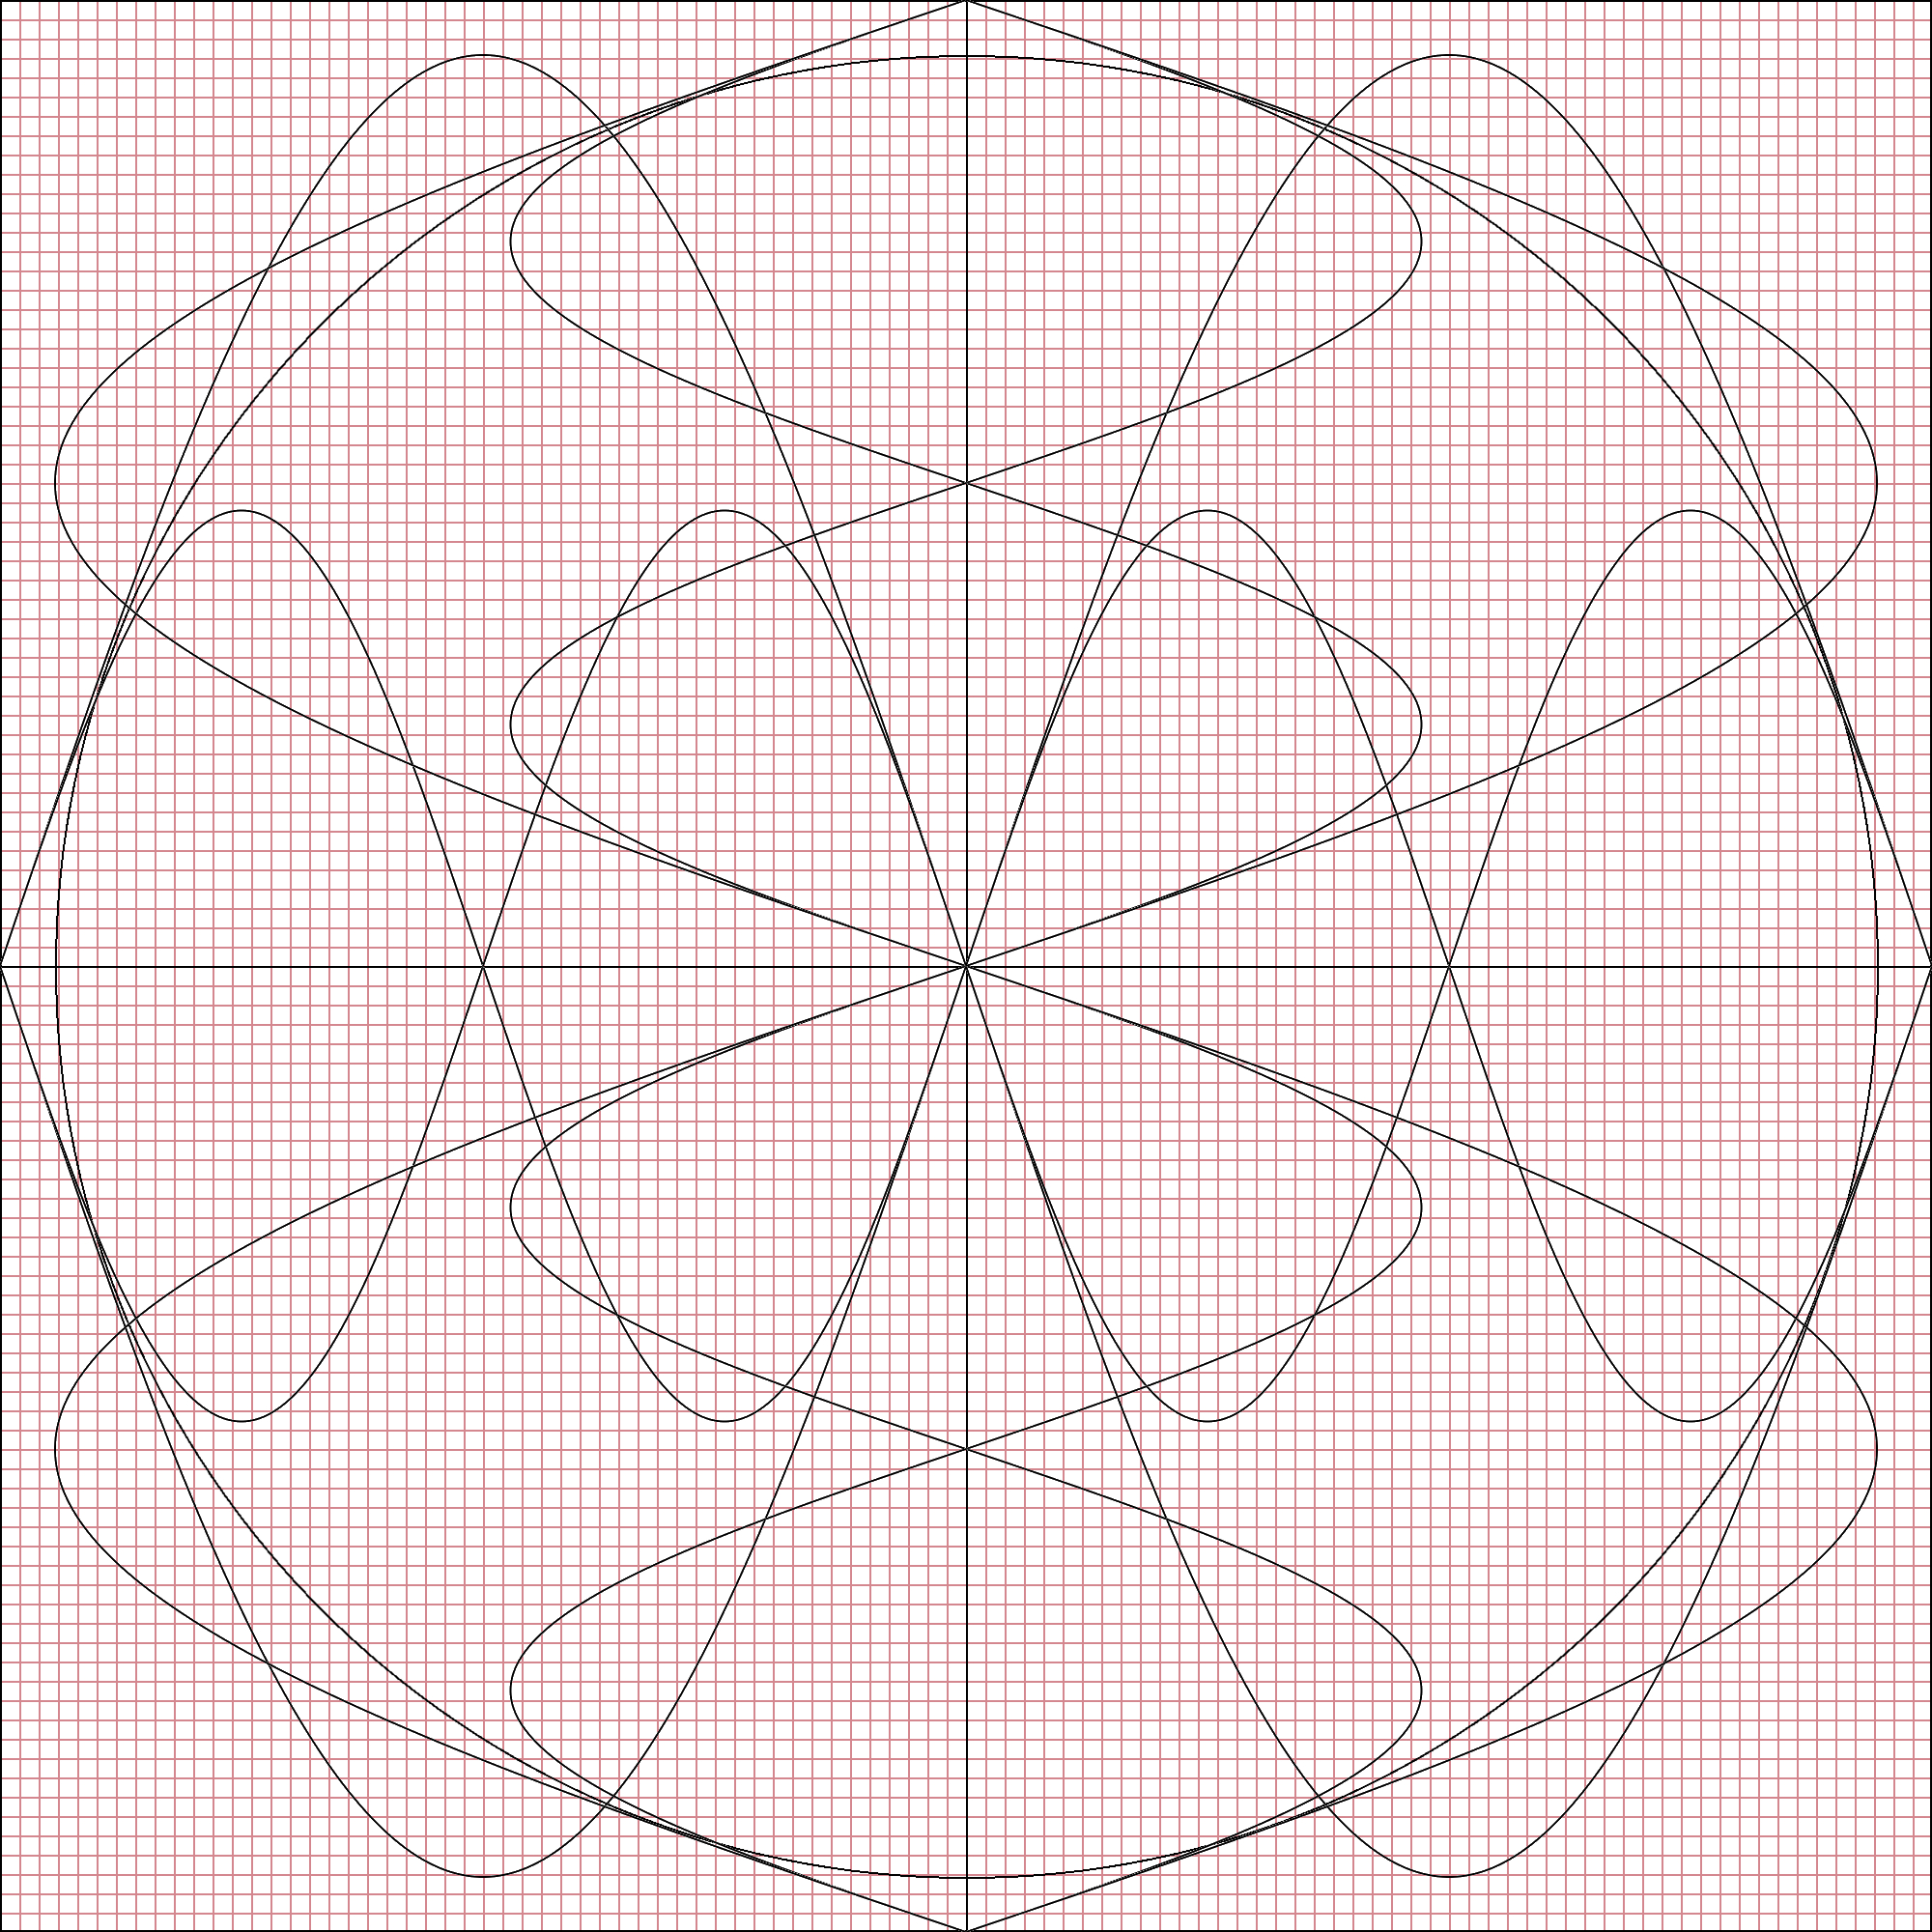
\includegraphics[width=.80\textwidth]{Front.jpg}
    \vfill
\end{titlepage}

\begin{abstract}
Wissenschaft ist der Versuch, Ordnung in das Unbekannte zu bringen.  
Sie sucht in allem Wandel nach den Konstanten, die bestehen bleiben,  
und in allem Zufall nach den Mustern, die ihn formen.  
Unter allen Disziplinen ist es die Physik,  
die diesen Anspruch am weitesten trägt:  
Sie beschreibt nicht nur, \emph{was} geschieht,  
sondern fragt, \emph{warum} es geschieht.  
\\
\noindent
Über Jahrhunderte hinweg wurde sie zum Fundament unseres Weltverständnisses.  
Sie zerlegte die Natur in Gesetze,  
maß Kräfte, Energien, Teilchen und Felder –  
und formte daraus ein Bild, das von beeindruckender Präzision ist.  
Doch trotz aller Erfolge blieb eines unvollendet:  
die Vereinigung ihrer eigenen Grundlagen.
\\
\noindent
Einstein erkannte, dass Raum und Zeit keine starren Koordinaten sind,  
sondern sich durch Energie und Masse krümmen.  
Seine Relativitätstheorie machte den Raum dynamisch,  
doch die Quantenmechanik sprach eine andere Sprache.  
Sie zeigte eine Welt, in der Wahrscheinlichkeiten regieren,  
in der Teilchen Wellen sind und Beobachtung Realität formt.  
Das Doppelspaltexperiment offenbarte dieses Paradox in seiner reinsten Form:  
Ein einzelnes Teilchen erzeugt ein Interferenzmuster,  
als ob es durch beide Spalte zugleich gegangen wäre.
\\
\noindent
Zwei Theorien, beide bewährt, beide richtig –  
und doch unvereinbar in ihrem Verständnis dessen,  
was sie beschreiben.  
Raum ist für die eine Bühne der Gravitation,  
für die andere nur der Hintergrund statistischer Zustände.  
Zwischen beiden liegt die größte Leerstelle der modernen Physik.
\noindent
\begin{center}
Eine Frage blieb bis heute unbeantwortet,  
und sie ist zugleich die einfachste und tiefste von allen:  
\end{center}

\vspace{2cm}
\begin{center}
    {\huge\textbf\emph{Was ist Raum?}}
\end{center}
\end{abstract}
\tableofcontents

\mainmatter
\input{content/01_einleitung}
\chapter{Mathematischer Rahmen I}
\begin{center}
    {\textbf{Die dreidimensionale Resonanzformulierung}}
\end{center}
\label{chap:mathematischer_rahmen_I}

\section{Einleitender Ansatz}

Das klassische
\textbf{Doppelspaltexperiment}
zeigt, dass die Trennung von Welle und Teilchen
keine physikalische Grundlage besitzt, sondern eine Folge unserer Beobachtung ist.
Wird die Beobachtungsebene selbst Teil der Betrachtung,
so zeigt sich, dass jedes Teilchenverhalten durch eine überlagerte Welle beschrieben werden kann.
Daraus ergibt sich die Annahme, dass Teilchen nichts anderes sind
als stabile Resonanzknoten solcher überlagerter Wellen,
deren Energieverteilung sich exponentiell in drei Dimensionen fortsetzt.
Jede dieser Überlagerungen bildet einen Knotenpunkt,
an dem sich Energie räumlich konzentriert. Dieser Knoten entspricht dem realen, beobachtbaren Teilchen.
\\
\begin{center}
    {\large\textbf{Mathematische Einschränkungen}}
\end{center}

Zur Beschreibung dieses Phänomens darf keine zweidimensionale Projektion mehr verwendet werden.
Jede Flächenbeschreibung (Kreise, Winkel, $\pi$-Bezüge)
reduziert den Raum auf eine irrationale Näherung, die keine physikalische Existenz besitzt.
Gesucht ist daher eine Operatorform,
die Raum, Energie und Zeit vollständig rational in drei Dimensionen verbindet.
Damit wird aus der Geometrie der Fläche eine Geometrie des Volumens,
deren Eigenschaften sich durch reale Messwerte bestätigen lassen müssen.

\section{Probleme zweidimensionaler Projektionen in der Physik}

Viele etablierte Gleichungen der Physik – insbesondere die Wellengleichung in ihrer Standardform –
setzen implizit eine zweidimensionale Geometrie voraus:
\[
\frac{\partial^2 \Psi}{\partial x^2} +
\frac{\partial^2 \Psi}{\partial y^2} = -k^2 \Psi.
\]
Diese Form beschreibt eine stehende Welle in einer Ebene,
nicht im realen Raum.
\newpage
\noindent
Die Erweiterung auf drei Dimensionen durch bloße Summation
\[
\nabla^2 \Psi =
\frac{\partial^2 \Psi}{\partial x^2} +
\frac{\partial^2 \Psi}{\partial y^2} +
\frac{\partial^2 \Psi}{\partial z^2}
\]
ändert daran nichts Wesentliches,
da sie den Raum als additive Kombination von Flächen behandelt.
Erst wenn der Operator selbst räumlich gekoppelt ist,
kann er reale Resonanzverhältnisse abbilden.

\section{Herleitung des Resonanzoperators}

Der Ausgangspunkt ist die klassische Wellengleichung
\[
\nabla^2 \Psi = \frac{1}{c^2} \frac{\partial^2 \Psi}{\partial t^2},
\]
die die zeitliche Ausbreitung einer Welle mit der räumlichen Krümmung ihres Feldes verknüpft.
Für stationäre Zustände der Energie gilt, dass sich die zeitliche Ableitung
als harmonische Oszillation der Form
\[
\Psi(\mathbf{x},t) = \psi(\mathbf{x}) e^{i\omega t}
\]
darstellen lässt.
Setzt man diesen Ausdruck in die Wellengleichung ein, ergibt sich nach Kürzung des Zeitfaktors
\[
\nabla^2 \psi + \frac{\omega^2}{c^2}\psi = 0.
\]
Dies ist die \gls{helmholtz} in ihrer Grundform.
Die auftretende Konstante
\[
k = \frac{\omega}{c}
\]
beschreibt hier keine klassische Wellenzahl im Sinne einer 2D-Projektion,
sondern das Verhältnis zwischen Energie und zeitlicher Resonanzfrequenz.
Damit kann man den allgemeinen Resonanzoperator definieren als
\[
\hat{R} = \nabla^2 + k^2,
\]
wobei $\hat{R}\psi = 0$ den stationären Zustand des Raumes beschreibt.
Dieser Operator verknüpft Raum und Zeit zu einer messbaren geometrischen Einheit
und wird in der Energie-Resonanz-Theorie als \emph{Raumresonanzoperator} bezeichnet.

\paragraph{Eigenschaften des Operators.}
Damit $\hat{R}$ eine reale, physikalische Bedeutung besitzt, muss er:
\begin{enumerate}
    \item \textbf{linear} sein, um Überlagerungen (Superposition) zuzulassen,
    \item \textbf{selbstadjungiert} sein, damit die Eigenwerte reell und beobachtbar bleiben,
    \item \textbf{räumlich symmetrisch} sein, um isotrope Resonanzen zu gewährleisten.
\end{enumerate}
Diese Eigenschaften führen zwingend dazu, dass nur reale, messbare Zustände
in der Lösungsmannigfaltigkeit vorkommen – die Theorie bleibt damit
vollständig empirisch anschlussfähig.

\section{Die drei Dimensionen der Realität}

In einem realen Resonanzraum existieren zu jeder Richtung zwei entgegengesetzte Ausbreitungsrichtungen.
Diese \gls{dualitaet} kann als Spiegelung der Energieflüsse verstanden werden.
Damit beschreibt der Laplace-Operator keine Summe unabhängiger Richtungen,
sondern eine gekoppelte Struktur:
\[
\nabla^2 \Psi =
\frac{\partial^2 \Psi}{\partial x_+^2} +
\frac{\partial^2 \Psi}{\partial x_-^2} +
\frac{\partial^2 \Psi}{\partial y_+^2} +
\frac{\partial^2 \Psi}{\partial y_-^2} +
\frac{\partial^2 \Psi}{\partial z_+^2} +
\frac{\partial^2 \Psi}{\partial z_-^2}.
\]
Hierbei stehen $(x_+,x_-)$, $(y_+,y_-)$ und $(z_+,z_-)$
für die dualen Ausbreitungsrichtungen der Raumdimensionen.
Diese Symmetrie beschreibt erstmals ein \emph{physikalisch geschlossenes Raumfeld},
in dem sich Energie als stehende dreidimensionale Welle stabilisiert.

\section{Robin-Randbedingungen als physikalische Kopplung}

An der Grenze eines Resonanzraumes darf Energie weder verloren gehen noch reflektionsfrei entweichen.
Diese Bedingung wird durch die \gls{robin} erfüllt:
\[
\frac{\partial \Psi}{\partial n} + \beta \Psi = 0,
\]
wobei der Parameter $\beta$ die Stärke der Kopplung zwischen Innen- und Außenraum beschreibt.
Der Term $\partial_n \Psi$ steht für den Energiefluss über die Raumgrenze,
$\beta \Psi$ für die Rückwirkung des umgebenden Resonanzfeldes.
Gemeinsam bilden beide Terme die physikalisch reale Stabilisierung eines Resonanzvolumens.

\section{Das entstehende Eigenwertproblem}

Wird der Operator $\hat{R}$ unter den Robin-Bedingungen gelöst,
so entsteht ein Eigenwertproblem der Form
\[
\hat{R}\Psi_i = \lambda_i \Psi_i,
\]
mit
\[
\nabla^2 \Psi_i + k_i^2 \Psi_i = 0, \quad
\frac{\partial \Psi_i}{\partial n} + \beta \Psi_i = 0.
\]
Die Eigenwerte $k_i$ repräsentieren die diskreten Resonanzzustände des Raumes.
Jeder \gls{eigenwert} steht für ein stabil existierendes Energieverhältnis,
das im physikalischen Raum beobachtbar sein muss.

\newpage

\subsection{Emergente Symmetrie der dreidimensionalen Randbedingung}

Die duale \gls{robin} erzwingt,
dass jede Welle sich in beiden Richtungen
entlang jeder Raumachse ausbreitet.
Damit entstehen \(2^3 = 8\)
mögliche Überlagerungsrichtungen.
Diese bilden die kleinstmögliche stabile
Resonanzeinheit der dreidimensionalen Geometrie.

Das resultierende \gls{achter-raster}
beschreibt die räumliche Diskretisierung,
die im folgenden Kapitel
zur numerischen Überprüfung herangezogen wird.

\section{Überleitung zum numerischen Experiment}

Das genannte Eigenwertproblem liefert die Grundlage für den empirischen Abgleich.
Durch numerische Lösung der Gleichung für verschiedene Randbedingungen
kann das Spektrum der Eigenwerte bestimmt werden.
Der folgende Schritt besteht darin,
diese berechneten Eigenwerte mit beobachtbaren Größen zu vergleichen
und nach einem konstanten Verhältnis zu suchen,
das alle Skalen miteinander verbindet.


\input{content/03_Numerischer_scan_fit}
\chapter{Mathematischer Teil II – Die Bedeutung von \gls{alpha-star}}
\label{chap:mathematischer_rahmen_II}

\section{Empirischer Bezug – Wechselspannung als Energie‐Zeit‐Symmetrie}

Im vorangegangenen Kapitel wurde gezeigt, dass sich durch numerische Rasterung
über acht Raumrichtungen hinweg ein konstanter Operator identifizieren lässt,
dessen Wert \gls{alpha-star} eine außergewöhnliche Skalenkonstanz über atomare,
nukleare und kosmologische Energiesysteme zeigt.
Um die physikalische Bedeutung dieses Operators zu klären,
bietet sich ein empirisch gut zugängliches Energiesystem an,
in dem Energie und Zeit periodisch gekoppelt sind:
das elektrische Wechselspannungsfeld.

\begin{figure}
  \centering
  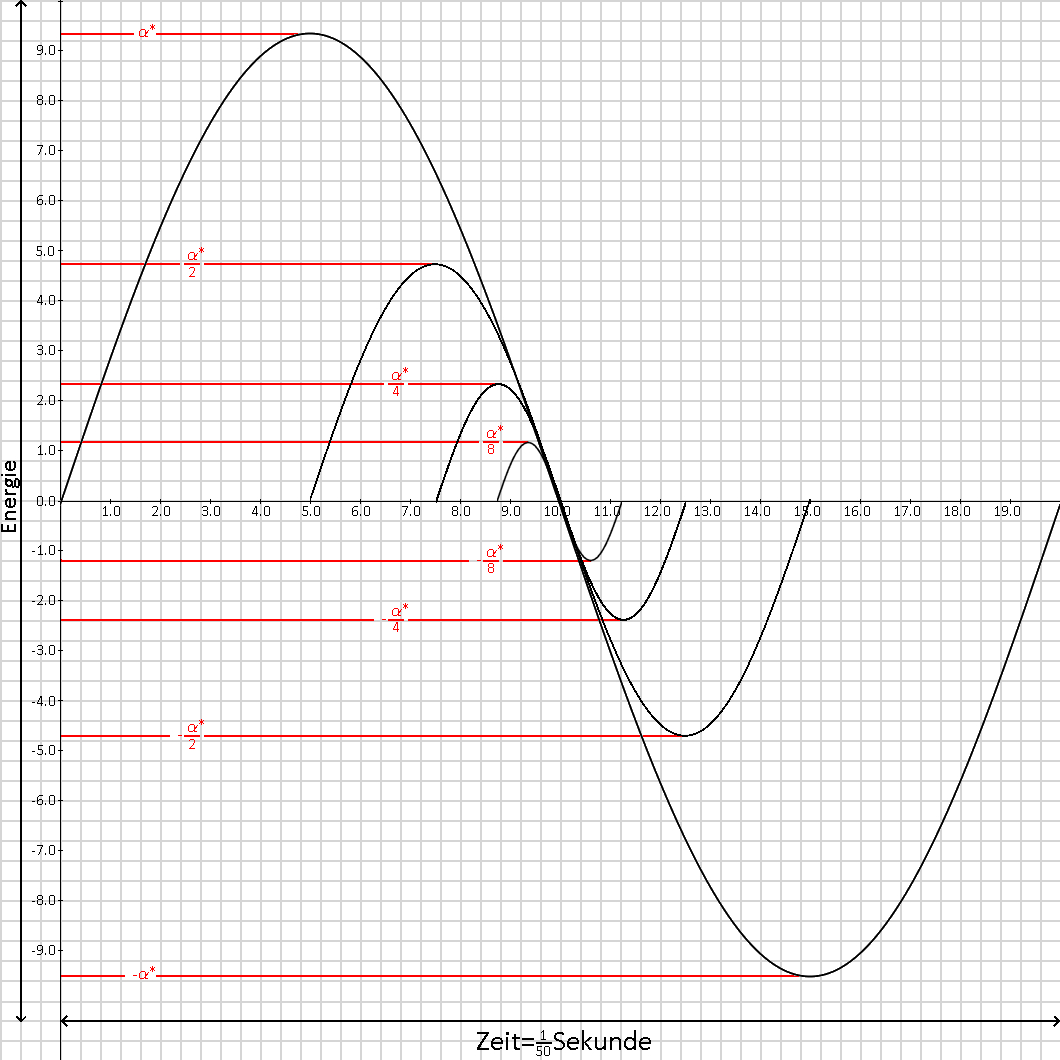
\includegraphics[width=0.85\textwidth]{Grafiken/Wechselspannung.jpg}
  \caption{Das normierte Wechselpannungsfeld enthält \gls{alpha-star}}
  \label{Diagramm1}
\end{figure}

Eine Wechselspannung beschreibt das zeitlich alternierende Potential
\[
U(t) = U_0 \sin(\omega t).
\]
Die Energie folgt dabei der quadratischen Form
\[
E(t) \propto U^2(t),
\]
wodurch sich eine periodische Energie–Zeit–Symmetrie ergibt.
Wird diese über mehrere Phasen hinweg verschoben,
entsteht eine geordnete, zeitlich und räumlich
symmetrische Energieverteilung.
Damit bildet die Wechselspannung eine natürliche Referenz
für das, was hier als \emph{aperiodische Energie–Zeit–Symmetrie}
der Realität verstanden wird.

Das elektrische Dreiphasensystem (Drehstrom)
stellt die empirische Analogie zum dreidimensionalen Raum dar:
drei zueinander phasenverschobene sinusförmige Potentiale,
deren gemeinsame Überlagerung eine stabile, rotierende
Energiekonfiguration erzeugt.
Dieses Verhalten deutet darauf hin, dass reale Energiesysteme
in drei Dimensionen einer übergeordneten geometrischen Symmetrie folgen,
in der Phasenwinkel und Raumrichtungen unmittelbar gekoppelt sind.

\section{Einführung des Operators \gls{alpha-star}}

Der empirische Fit über verschiedene Energieskalen
führte auf einen dimensionslosen Operator
\[
\alpha^* = 9{,}43034098\dots
\]
der in allen getesteten Domänen (atomar, nuklear, kosmologisch)
als skalierungsstabiler Eigenwert auftritt.
In energetischer Interpretation beschreibt \gls{alpha-star}
ein konstantes Verhältnis von Energie zu Zeit.
Formal lässt sich schreiben:
\[
\alpha^* = \frac{E}{T},
\]
wobei $E$ die mittlere Energiedichte
und $T$ der effektive Zeitintervall der \gls{resonanz} ist.
Damit wird \gls{alpha-star} zur \emph{energetischen Frequenzkonstante}
des Raumes selbst.

\section{Das Dreiphasensystem und der Winkelbezug}

Überträgt man den Befund auf das Dreiphasensystem,
so zeigt sich, dass drei periodische Signale
\[
U_i(t) = U_0 \sin(\omega t + \phi_i),
\qquad
\phi_i = \{0,\,120^\circ,\,240^\circ\}
\]
ein vollständiges symmetrisches Energiesystem bilden.
Dieses System erzeugt eine rotierende Feldstruktur,
die in allen drei Raumrichtungen denselben Energieverlauf besitzt.
Die 120°‐Phasenverschiebung lässt sich dabei
als projektiver Anteil eines übergeordneten Öffnungswinkels interpretieren.
Setzt man \gls{alpha-star} in Relation zur vollen Kreisphase $360^\circ$,
so ergibt sich
\[
\frac{\alpha^*}{360^\circ} = 0{,}0261953916\dots
\]
und der daraus abgeleitete Öffnungswinkel
\[
\theta^* = 360^\circ \cdot \frac{\alpha^*}{10} = 20{,}50772472^\circ.
\]
Dieser Winkel beschreibt die aperiodische Abweichung
von einer idealen Periode 10
und bildet somit die geometrische Interpretation
des empirisch gefundenen Operators.

\section{Herleitung der \gls{spiralis}‐Funktion mit \gls{alpha-star}}

Die klassische Sinusfunktion
\[
s(\xi) = \sin(2\pi\,\xi)
\]
beschreibt eine periodische Schwingung in einer Dimension.
Für reale Energiesysteme muss jedoch berücksichtigt werden,
dass Raum und Zeit untrennbar gekoppelt sind
und die Schwingung nicht in einer Ebene,
sondern entlang einer räumlichen Spirale verläuft.
Diese Spiralität führt zur beobachteten \gls{aperiodizitaet} der Realität.

Die \emph{\gls{spiralis}‐Funktion} verallgemeinert den Sinus
auf einen aperiodischen, dreidimensionalen Verlauf.
Dazu wird die Phase nicht mehr durch $2\pi$ bestimmt,
sondern durch den empirischen Öffnungswinkel \gls{alpha-star}.
Für eine Dimension ergibt sich:
\[
\mathcal{S}_1(x) = \sin\!\left(\frac{\alpha^*}{3}x\right),
\]
für zwei Dimensionen:
\[
\mathcal{S}_2(x,y) = \sin\!\left(\frac{\alpha^*}{2}(x+y)\right),
\]
und für drei Dimensionen:
\[
\boxed{
\mathcal{S}_3(x,y,z)
= \sin\!\left(\alpha^*\,(x+y+z)\right).
}
\]
Die dreidimensionale \gls{spiralis} bildet damit
die energetische Grundform des Raumes.
Ihre \gls{aperiodizitaet} erklärt,
warum keine natürlichen Systeme exakt periodisch erscheinen
und warum reale Resonanzen stets einen Spiralcharakter besitzen.

\section{Eigenschaften und Bedeutung der \gls{spiralis}‐Geometrie}

Die \gls{spiralis}‐Geometrie besitzt mehrere bemerkenswerte Eigenschaften:

\begin{enumerate}
\item \textbf{\gls{aperiodizitaet}:}
Die Funktion wiederholt sich nicht exakt;
sie nähert sich einer Periode nur asymptotisch.
Dies spiegelt das Verhalten realer Umlaufbahnen,
Rotationen und Schwingungen wider.

\item \textbf{Symmetrie:}
In drei Dimensionen ergeben sich acht stabile Richtungen
(Octants), in denen die \gls{spiralis}‐Welle
überlagerungsstabil ist.
Dies führt zur beobachteten 8‐fachen Symmetrie
in den numerischen Simulationen.

\item \textbf{Hierarchie:}
Durch Überlagerung mehrerer \gls{spiralis}‐Knoten
unterschiedlicher Ordnung entstehen komplexe Strukturen
– von atomaren Feldern bis zu makroskopischer Materie.
Ein einfaches Beispiel ist die Kopplung zweier
dreidimensionaler \gls{spiralis}‐Felder entlang einer Achse,
die das Verhalten des Wasserstoffmoleküls H$_2$ reproduziert.

\item \textbf{Projektion:}
In eindimensionaler Projektion
erscheint die \gls{spiralis} als klassische Sinuswelle;
die Kreisform (und damit $\pi$) ist
nur eine zweidimensionale Projektion
der aperiodischen Spiralbewegung in drei Dimensionen.
\end{enumerate}

Damit wird \gls{alpha-star} zum zentralen Operator,
der die Kopplung von Energie, Raum und Zeit
in einem aperiodischen, aber strukturerhaltenden
dreidimensionalen Resonanzfeld beschreibt.

\chapter{Visuelles Experiment – Numerische Überprüfung der Spiralis-Funktion}
\label{chap:visualisierung}

Nach der Herleitung der Spiralis-Funktion in Kapitel~\ref{chap:mathematischer_rahmen_II}
folgt nun ein zweiter, unabhängiger experimenteller Prüfstein.
Da sich die resultierende Geometrie nicht mehr intuitiv vorstellen lässt,
wird ein numerisches Visualisierungsexperiment durchgeführt, um die räumliche
Energieverteilung der Spiralis-Funktion darzustellen und zu analysieren.

\section{Zielsetzung und Methodik}

Ziel dieses Experiments ist es, zu überprüfen, ob die in Kapitel~\ref{chap:mathematischer_rahmen_II}
definierte Funktion in der Lage ist, reales Energieverhalten im Raum
darzustellen und als Volumen zu berechnen.
Das Experiment dient damit als numerischer Beweis der geometrischen Konsistenz
der Spiralis-Funktion.

Dazu werden zwei Werkzeuge eingesetzt:
\begin{itemize}
  \item \textbf{Python} als numerischer Operator, der die Funktion in einem
        diskreten kartesischen Gitter berechnet, die Werte auf den Bereich
        $[0,1]$ normalisiert und als Voxel-Datensatz im \texttt{.vti}-Format
        abspeichert;
  \item \textbf{\gls{paraview}} als dreidimensionaler Renderingraum, in dem die
        Volumendaten visuell analysiert und farbcodiert dargestellt werden.
\end{itemize}

Als Farbcodierung wird die empirisch abgeleitete elektromagnetische Farbskala
(\emph{EM-Colormap}) verwendet, die sich vom ultravioletten bis zum
infraroten Spektralbereich erstreckt.
Damit lässt sich die Energieverteilung in allen Bereichen des Volumens
kontinuierlich abbilden.

\section{Farbraum und Wahrnehmung}

Die für das visuelle Experiment verwendete Colormap \texttt{ERT\_EM\_Colormap} 
ist direkt aus den spektralen Eigenschaften des elektromagnetischen Feldes 
hergeleitet. Sie dient nicht als bloßes Darstellungswerkzeug, 
sondern als empirisch kohärente Übersetzung zwischen 
dem physikalischen Informationsfeld der Spiralis 
und der menschlichen Farbwahrnehmung.

\subsection{Sphärische Projektion des elektromagnetischen Spektrums}

Das sichtbare Licht wird in der Realität als schmaler Ausschnitt des 
elektromagnetischen Spektrums erfahren. In der Energieresonanz-Theorie wird 
dieser Bereich als der positive Teil der Spiralis interpretiert, 
dessen informatives Zentrum bei $u = 0{,}75$ liegt. 
Dieser Punkt markiert den Farbbereich \emph{Grün} als symmetrische Mitte 
der Wahrnehmungsskala, da er sowohl in Richtung kürzerer (violett/UV) 
als auch längerer (rot/IR) Wellenlängen die gleiche strukturelle Distanz besitzt. 

Die Colormap wird daher nicht linear, sondern \emph{sphärisch} aufgebaut:
sie bildet die wahrnehmbare Energiestruktur so ab, 
dass Schwarz und Weiß die Grenzen der periodisierten Wahrnehmung darstellen,
während alle Farben dazwischen aus der Spiralis hervorgehen. 
Mathematisch ist sie definiert als Abbildung
\[
C(u): [0,1] \to \mathbb{R}^3, \qquad 
C(u) = \bigl(R(u),G(u),B(u)\bigr),
\]
mit diskreten, experimentell gesetzten "RGBPoints":
\[
\begin{array}{rclcl}
u=0.000000   &\rightarrow& \text{Schwarz (Raum)} \ &\;& R=G=B=0, \\[2pt]
u=0.500000   &\rightarrow& \text{Schwarz-UV}\ &\;& R=G=B=0, \\[2pt]
u=0.556965  &\rightarrow& \text{Violett}\ &\;& R=0.5\ G=0\ B=1, \\[2pt]
u=0.653482  &\rightarrow& \text{Blau}\ &\;& R=G=0\ B=1, \\[2pt]
u=0.701741  &\rightarrow& \text{Cyan}\ &\;& R=0\ G=B=1, \\[2pt]
u=0.725870  &\rightarrow& \text{Grün}\ &\;& R=0\ G=1\ B=0, \\[2pt]
u=0.774129  &\rightarrow& \text{Grün}\ &\;& R=0\ G=1\ B=0, \\[2pt]
u=0.798258   &\rightarrow& \text{Gelb}\ &\;& R=G=1\ B=0, \\[2pt]
u=0.846517   &\rightarrow& \text{Orange}\ &\;& R=1\ G=0.5\ B=0, \\[2pt]
u=0.943034   &\rightarrow& \text{rot}\ &\;& R=1\ G=B=0, \\[2pt]
u=1.000000   &\rightarrow& \text{IR-Weiß}\ &\;& R=G=B=1, \\[2pt]
\end{array}
\]

\subsection{Kohärenz zur Farbwahrnehmung}

Die gewählten Punkte entsprechen nicht einer linearen Interpolation 
von Wellenlängen, sondern folgen der aperiodischen Symmetrie der Spiralis.  
Der Übergang von $u=0{,}556965$ bis $u=0{,}943034098=\frac{\alpha^*}{10}$
beschreibt den sichtbaren Ausschnitt des Feldes; 
die Bereiche unterhalb bzw.\ oberhalb bilden 
die unsichtbaren UV- und IR-Zonen, die vom Wahrnehmungssystem 
durch Opazität $\tau=0$ ausgeblendet werden.  
Damit stimmt die Colormap strukturell exakt mit der menschlichen Wahrnehmung überein:
das Gehirn „normalisiert“ die unendliche Farbskala ebenso auf ein Fenster
zwischen Schwarz und Weiß.

\subsection{Symbolische Interpretation}

Schwarz und Weiß markieren die beiden Pole des Resonanzfeldes:
Schwarz steht für das informativ unbestimmte Minimum 
(Nullresonanz, Raumanteil), 
Weiß für die vollständige Überlagerung aller Frequenzen 
(Maximalresonanz, Energieanteil).  
Die farbige Zone dazwischen stellt den periodischen, 
erfahrbaren Teil der Realität dar.  
Somit ist die Colormap nicht nur ein technisches Werkzeug, 
sondern ein direktes Abbild der 
\emph{energetischen Projektion der Realität} 
im Rahmen der Energieresonanz-Theorie.



\subsection{\gls{normalisierung} und Wahrnehmung}

Vor der Visualisierung wird das berechnete Volumen auf den Wertebereich $[0,1]$
normalisiert:
\[
F_\text{norm} = \frac{F - F_\text{min}}{F_\text{max} - F_\text{min}}.
\]
Diese \gls{normalisierung} ist notwendig, um sowohl in der Visualisierung
(\gls{paraview}) als auch in der Wahrnehmung des Beobachters
eine konsistente Interpretation zu ermöglichen.
Sie entspricht der optischen Kalibrierung eines realen Sensors.

\section{Numerische Implementierung des Generator-Skripts}

Das in diesem Abschnitt verwendete Skript \texttt{generator\_final.py} bildet den Kern des numerischen Versuchs. Es erzeugt sämtliche Volumendaten (\texttt{.vti}-Dateien) des Experiments — \textit{Proton}, \textit{H}, \textit{H\textsubscript{2}}, \textit{O} und \textit{H\textsubscript{2}O} — ausschließlich auf Grundlage der Spiralis-Funktion. Der Code generiert diese Volumen hierarchisch und gekoppelt, sodass jede Stufe die energetische Überlagerung der vorhergehenden beschreibt.

Das Skript folgt der in Kapitel~2 eingeführten \gls{helmholtz} mit Robin-Randbedingungen und verwendet die in Kapitel~4 definierte Operatorstruktur \(\alpha^*\) als numerischen Parameter. Die Feldwerte werden auf einem kartesischen Gitter normalisiert und nach der Relation
\[
\Psi(x,y,z) = \sin\!\bigl(\alpha^*(x+y+z)\bigr)
\]
berechnet. Die resultierende dreidimensionale Energiedichte wird in \texttt{.vti}-Dateien gespeichert und anschließend mit \gls{paraview} volumetrisch dargestellt.

Der hierarchische Aufbau folgt den Resonanzstufen:
\begin{itemize}
  \item \textbf{Proton:} erste stabile Spiralis-Überlagerung (Basisebene)
  \item \textbf{H:} achtfache Kopplung des Protons
  \item \textbf{H\textsubscript{2}:} eindimensionale Resonanzkopplung zweier H-Felder
  \item \textbf{O:} höhere hierarchische Ordnung der H-Struktur
  \item \textbf{H\textsubscript{2}O:} dreidimensionale Kopplung von H und O zur stabilsten Resonanzform
\end{itemize}

Alle Simulationen erfolgen im selben Koordinatenrahmen, identischer Auflösung und identischen Kameraparametern, um die energetischen Unterschiede ausschließlich aus der Feldstruktur selbst entstehen zu lassen. Die visuelle Darstellung erfolgt mit der in diesem Kapitel definierten \textit{EM-Colormap}, die die wahrnehmbare Energieverteilung des elektromagnetischen Spektrums abbildet.

\newpage

\section{Ergebnisse und Beobachtungen}
In diesem Abschnitt werden die visuellen Ergebnisse des numerischen Experiments vorgestellt und in ihrer hierarchischen Abfolge analysiert.
Jede Visualisierung basiert auf der identischen numerischen Basis der Spiralis-Funktion und unterscheidet sich ausschließlich durch den hierarchischen Kopplungsgrad der \gls{resonanz}. 
Die verwendete \textit{EM-Colormap} bildet dabei das wahrnehmbare elektromagnetische Spektrum ab und erlaubt eine unmittelbare Zuordnung zwischen mathematischem Feld und menschlicher Farbwahrnehmung. 
Die Kameraposition, Auflösung und \gls{normalisierung} bleiben über alle Datensätze hinweg konstant, um eine vergleichbare Darstellung der energetischen Geometrien zu gewährleisten.
\\
\\
Die jeweilige .vti-Datei wird in Paraview geladen, als Volume dargestellt und nutzt die Colormap als Farbgebung der Energieverteilung.
\\
\\
Alle Bilder sind Screenshots der gerenderten Volumen mit diesen Einstellungen und der selben Kameraperspektive.

\newpage

\subsection{Das Proton}

\begin{figure}
  \centering
  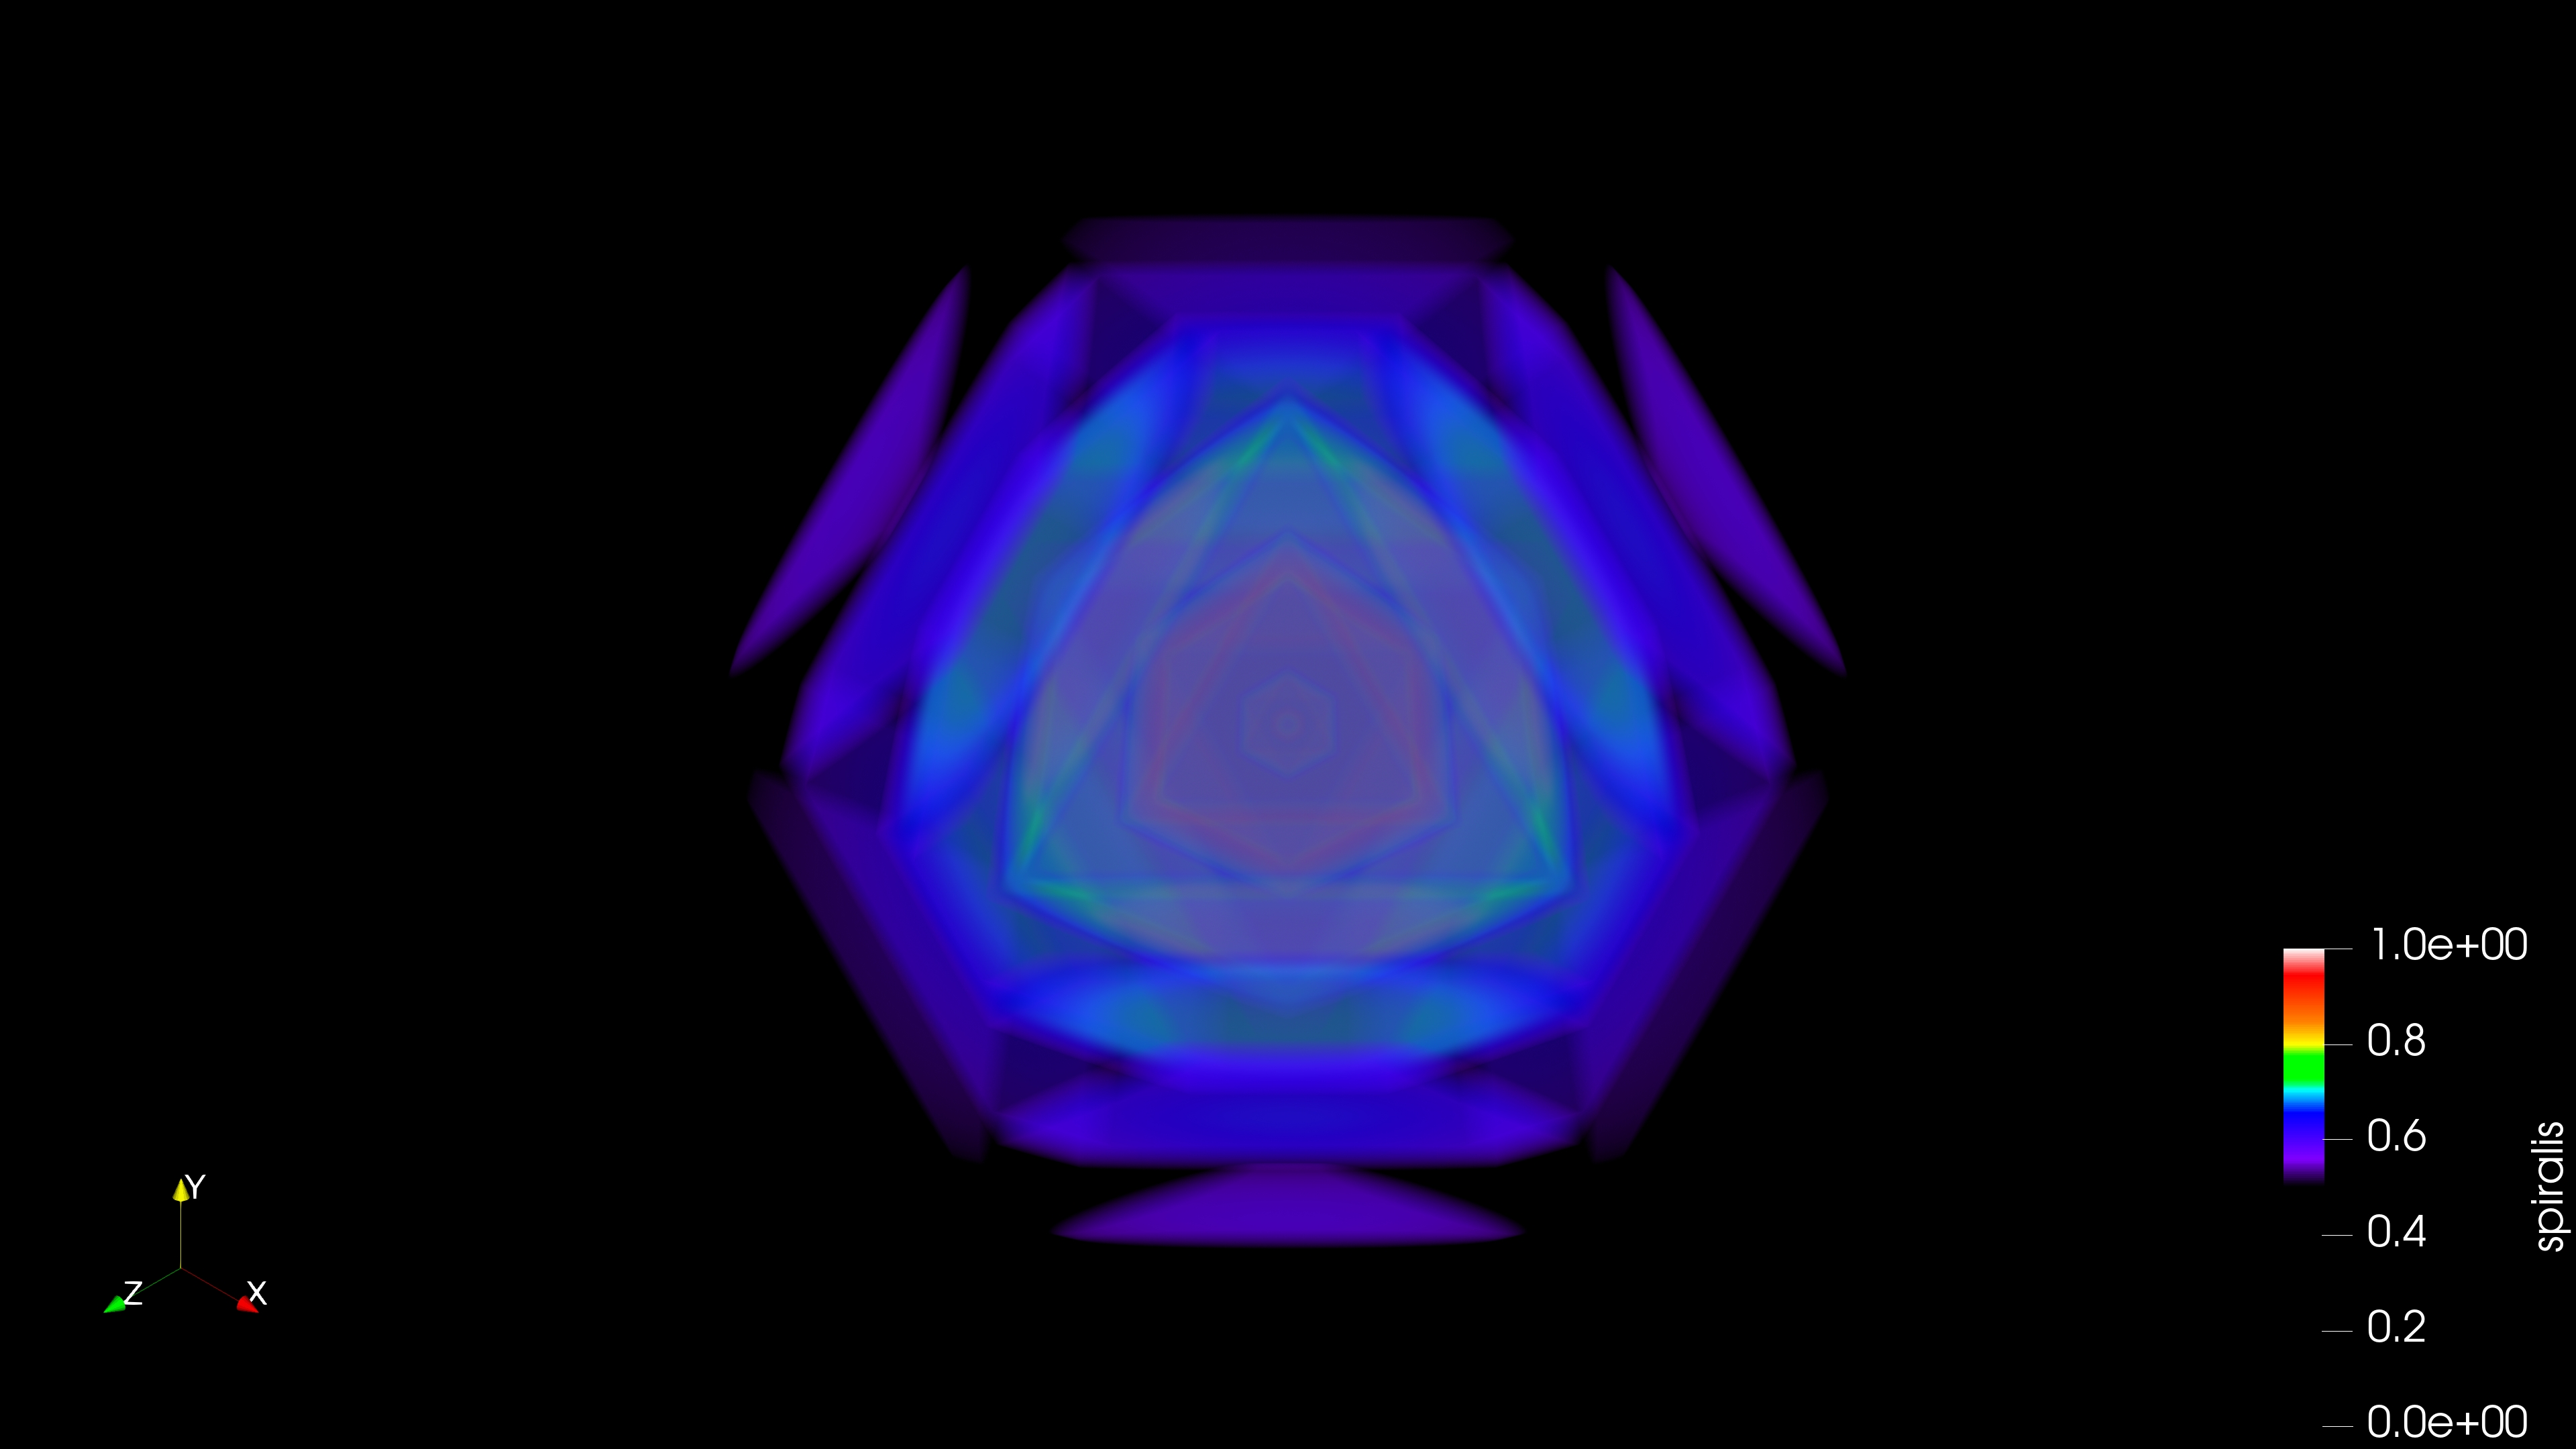
\includegraphics[width=0.85\textwidth]{Grafiken/05_Visualisierung/Proton/Proton_Volume_XYZ_Cam.jpeg}
  \caption{Darstellung der Proton.vti-Datei in Paraview}
  \label{fig:proton}
\end{figure}

Die erste stabile Spiralis-Struktur entsteht bei der achtfachen Raumüberlagerung. 
Sie bildet den energetischen Grundzustand des Feldes und markiert den ersten stationären Knoten der Raumenergie.
Das charakteristische Muster zeigt eine \emph{achtfache Symmetrie} um das Zentrum, die sich in allen höheren Strukturen wiederfindet. 
Die Visualisierung verdeutlicht die Stabilität dieser Anordnung — die Raumenergie faltet sich entlang der drei Raumachsen zu einem energetisch geschlossenen Knoten.
Der innere Bereich erscheint als konzentriertes, sphärisches Leuchten mit klarer Abgrenzung zum umgebenden Resonanzraum.
Das Proton stellt somit die elementare, selbststabilisierte Raumenergieeinheit dar.

\newpage

\subsection{Das Wasserstoffatom (H)}

\begin{figure}
  \centering
  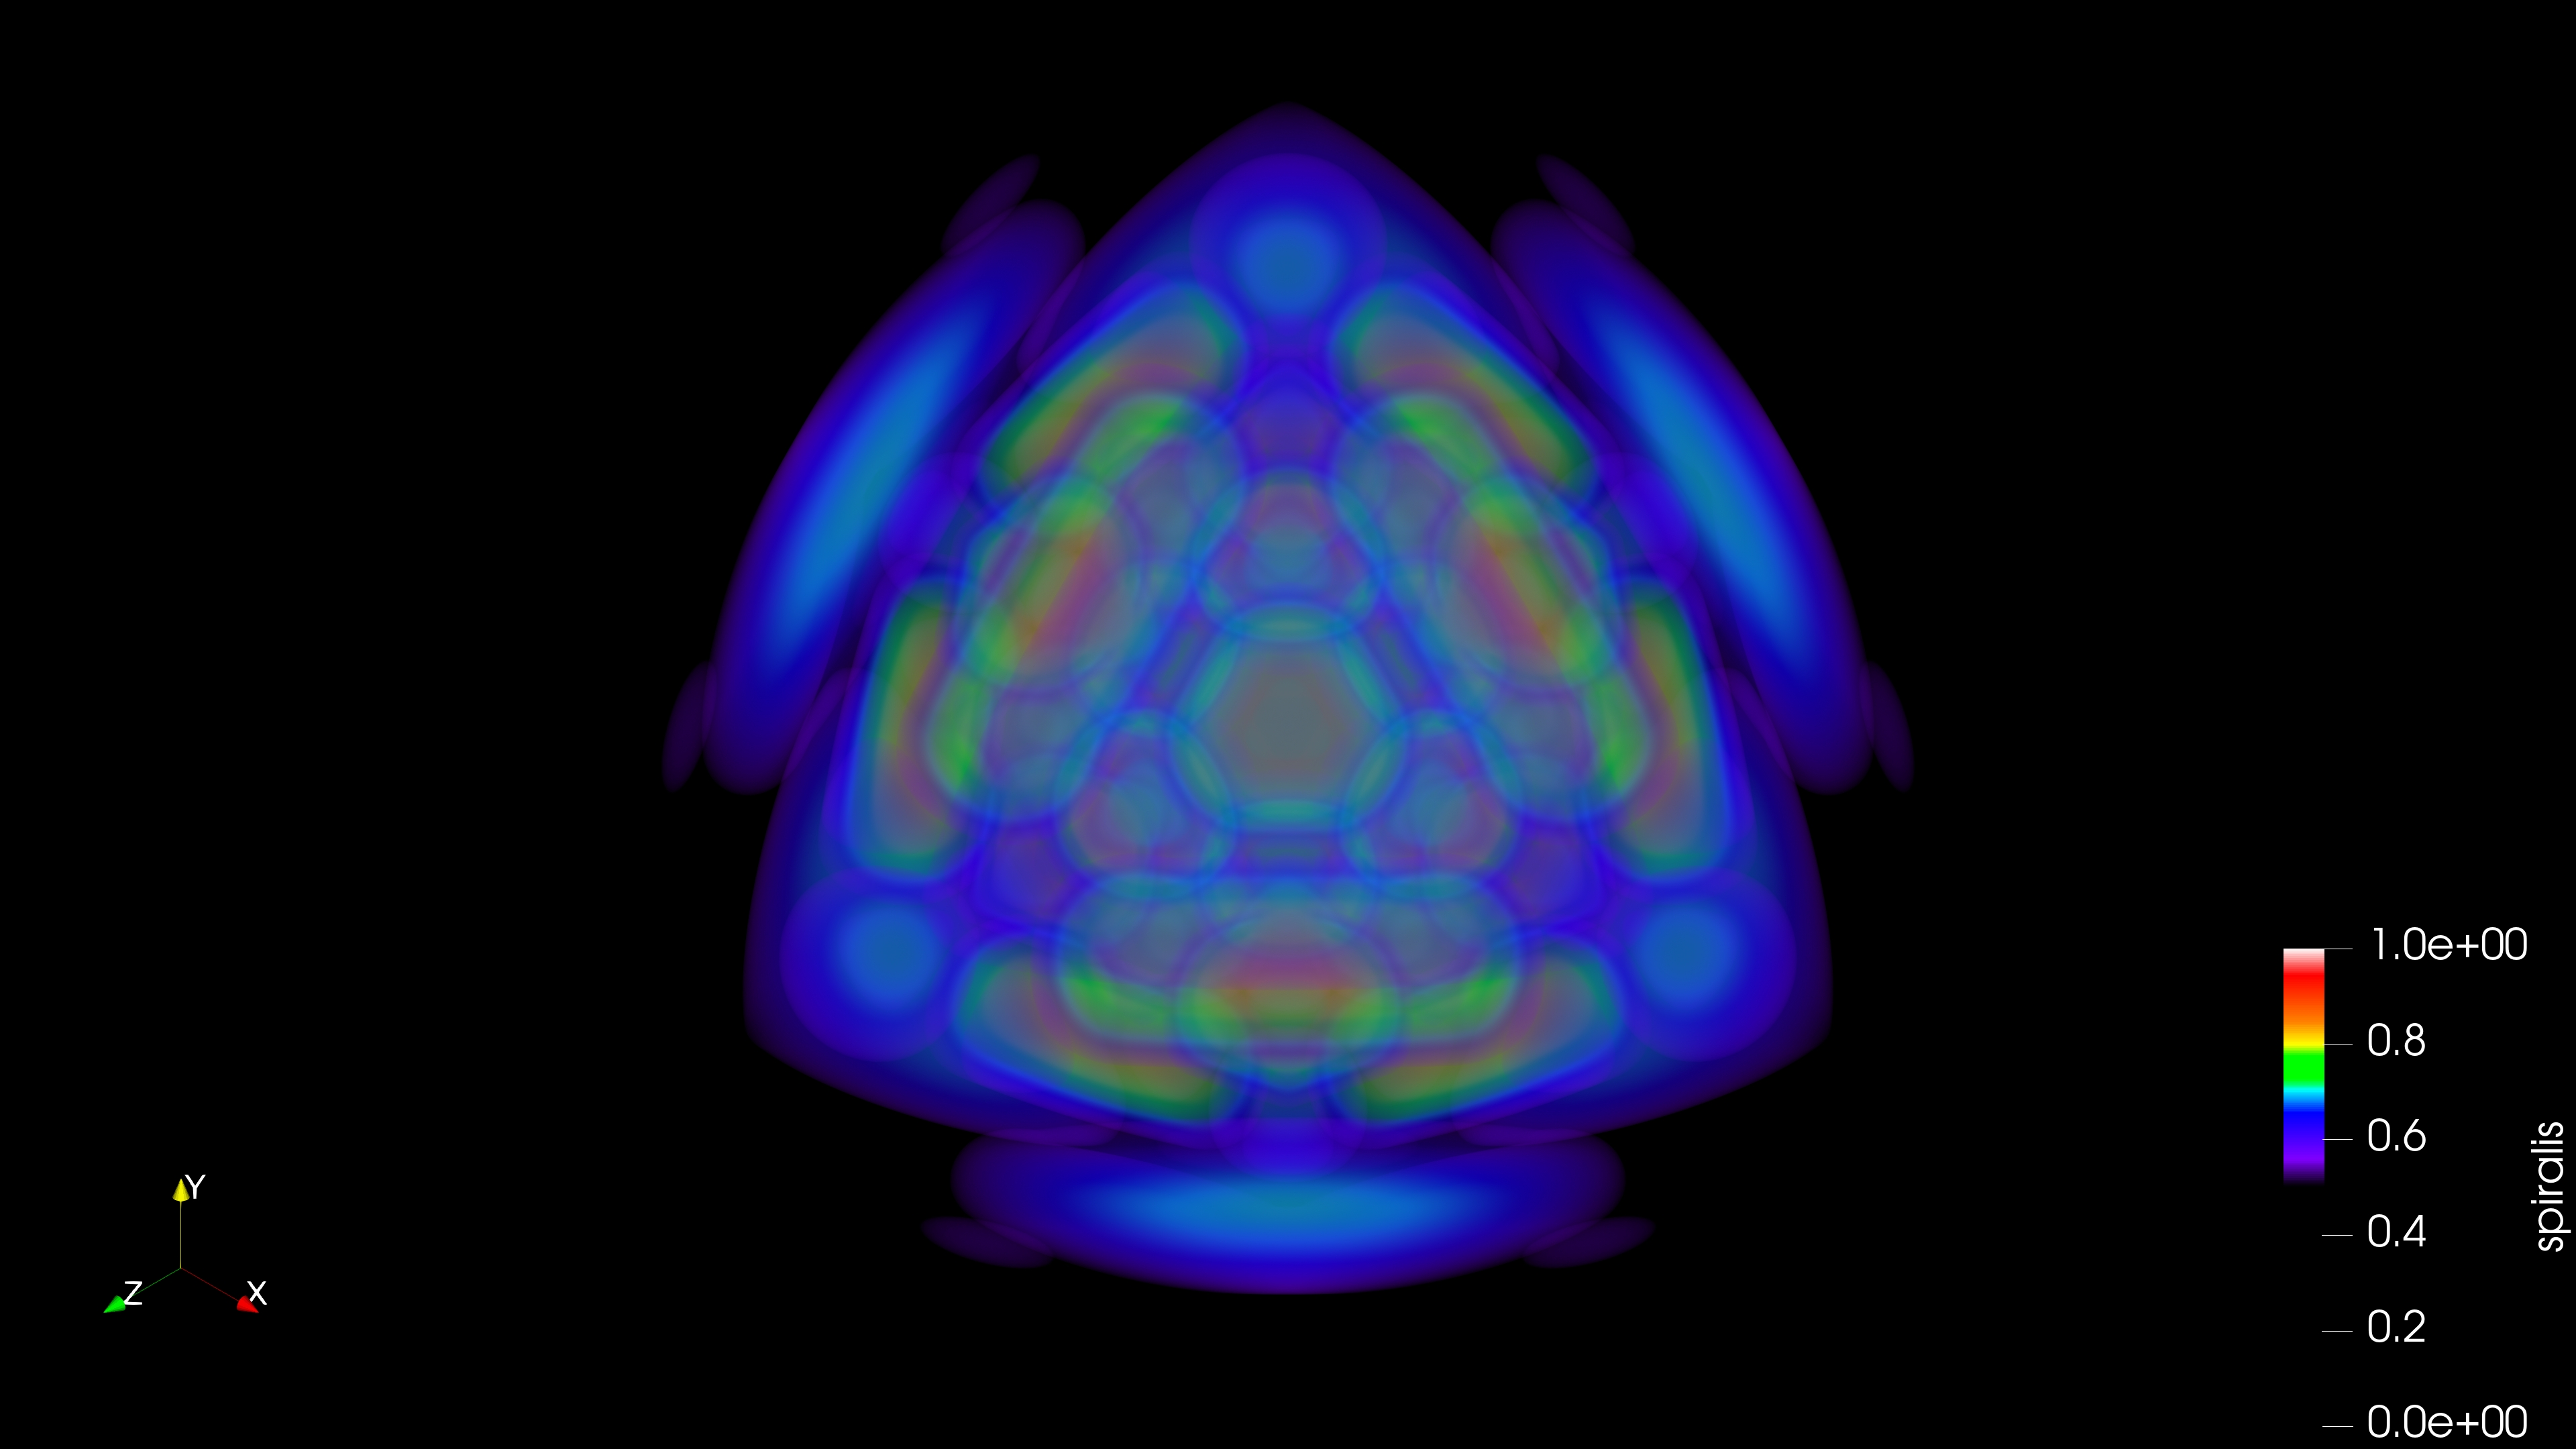
\includegraphics[width=0.85\textwidth]{Grafiken/05_Visualisierung/H/H_Volume_XYZ_Cam.jpeg}
  \caption{Darstellung der H.vti-Datei in Paraview}
  \label{fig:H}
\end{figure}

Durch achtfache Kopplung der Protonstruktur entsteht eine neue, räumlich erweiterte Energiedichteverteilung. 
Die Spiralis-Überlagerungen formen eine nahezu kugelsymmetrische Feldverteilung, deren Kern eine deutliche Steigerung der Energieintensität zeigt. 
Die Übergänge zwischen innerem und äußerem Feldbereich verlaufen harmonisch und erzeugen das typische visuelle Erscheinungsbild eines atomaren Energiepotentials.
Im Gegensatz zum Proton ist die Struktur hier bereits in der Lage, energetische Wechselwirkungen aufzunehmen, was sich in einer deutlichen Durchdringung des Raumfeldes zeigt.

\newpage

\subsection{Die Wasserstoffmolekülbindung (H2)}

\begin{figure}
  \centering
  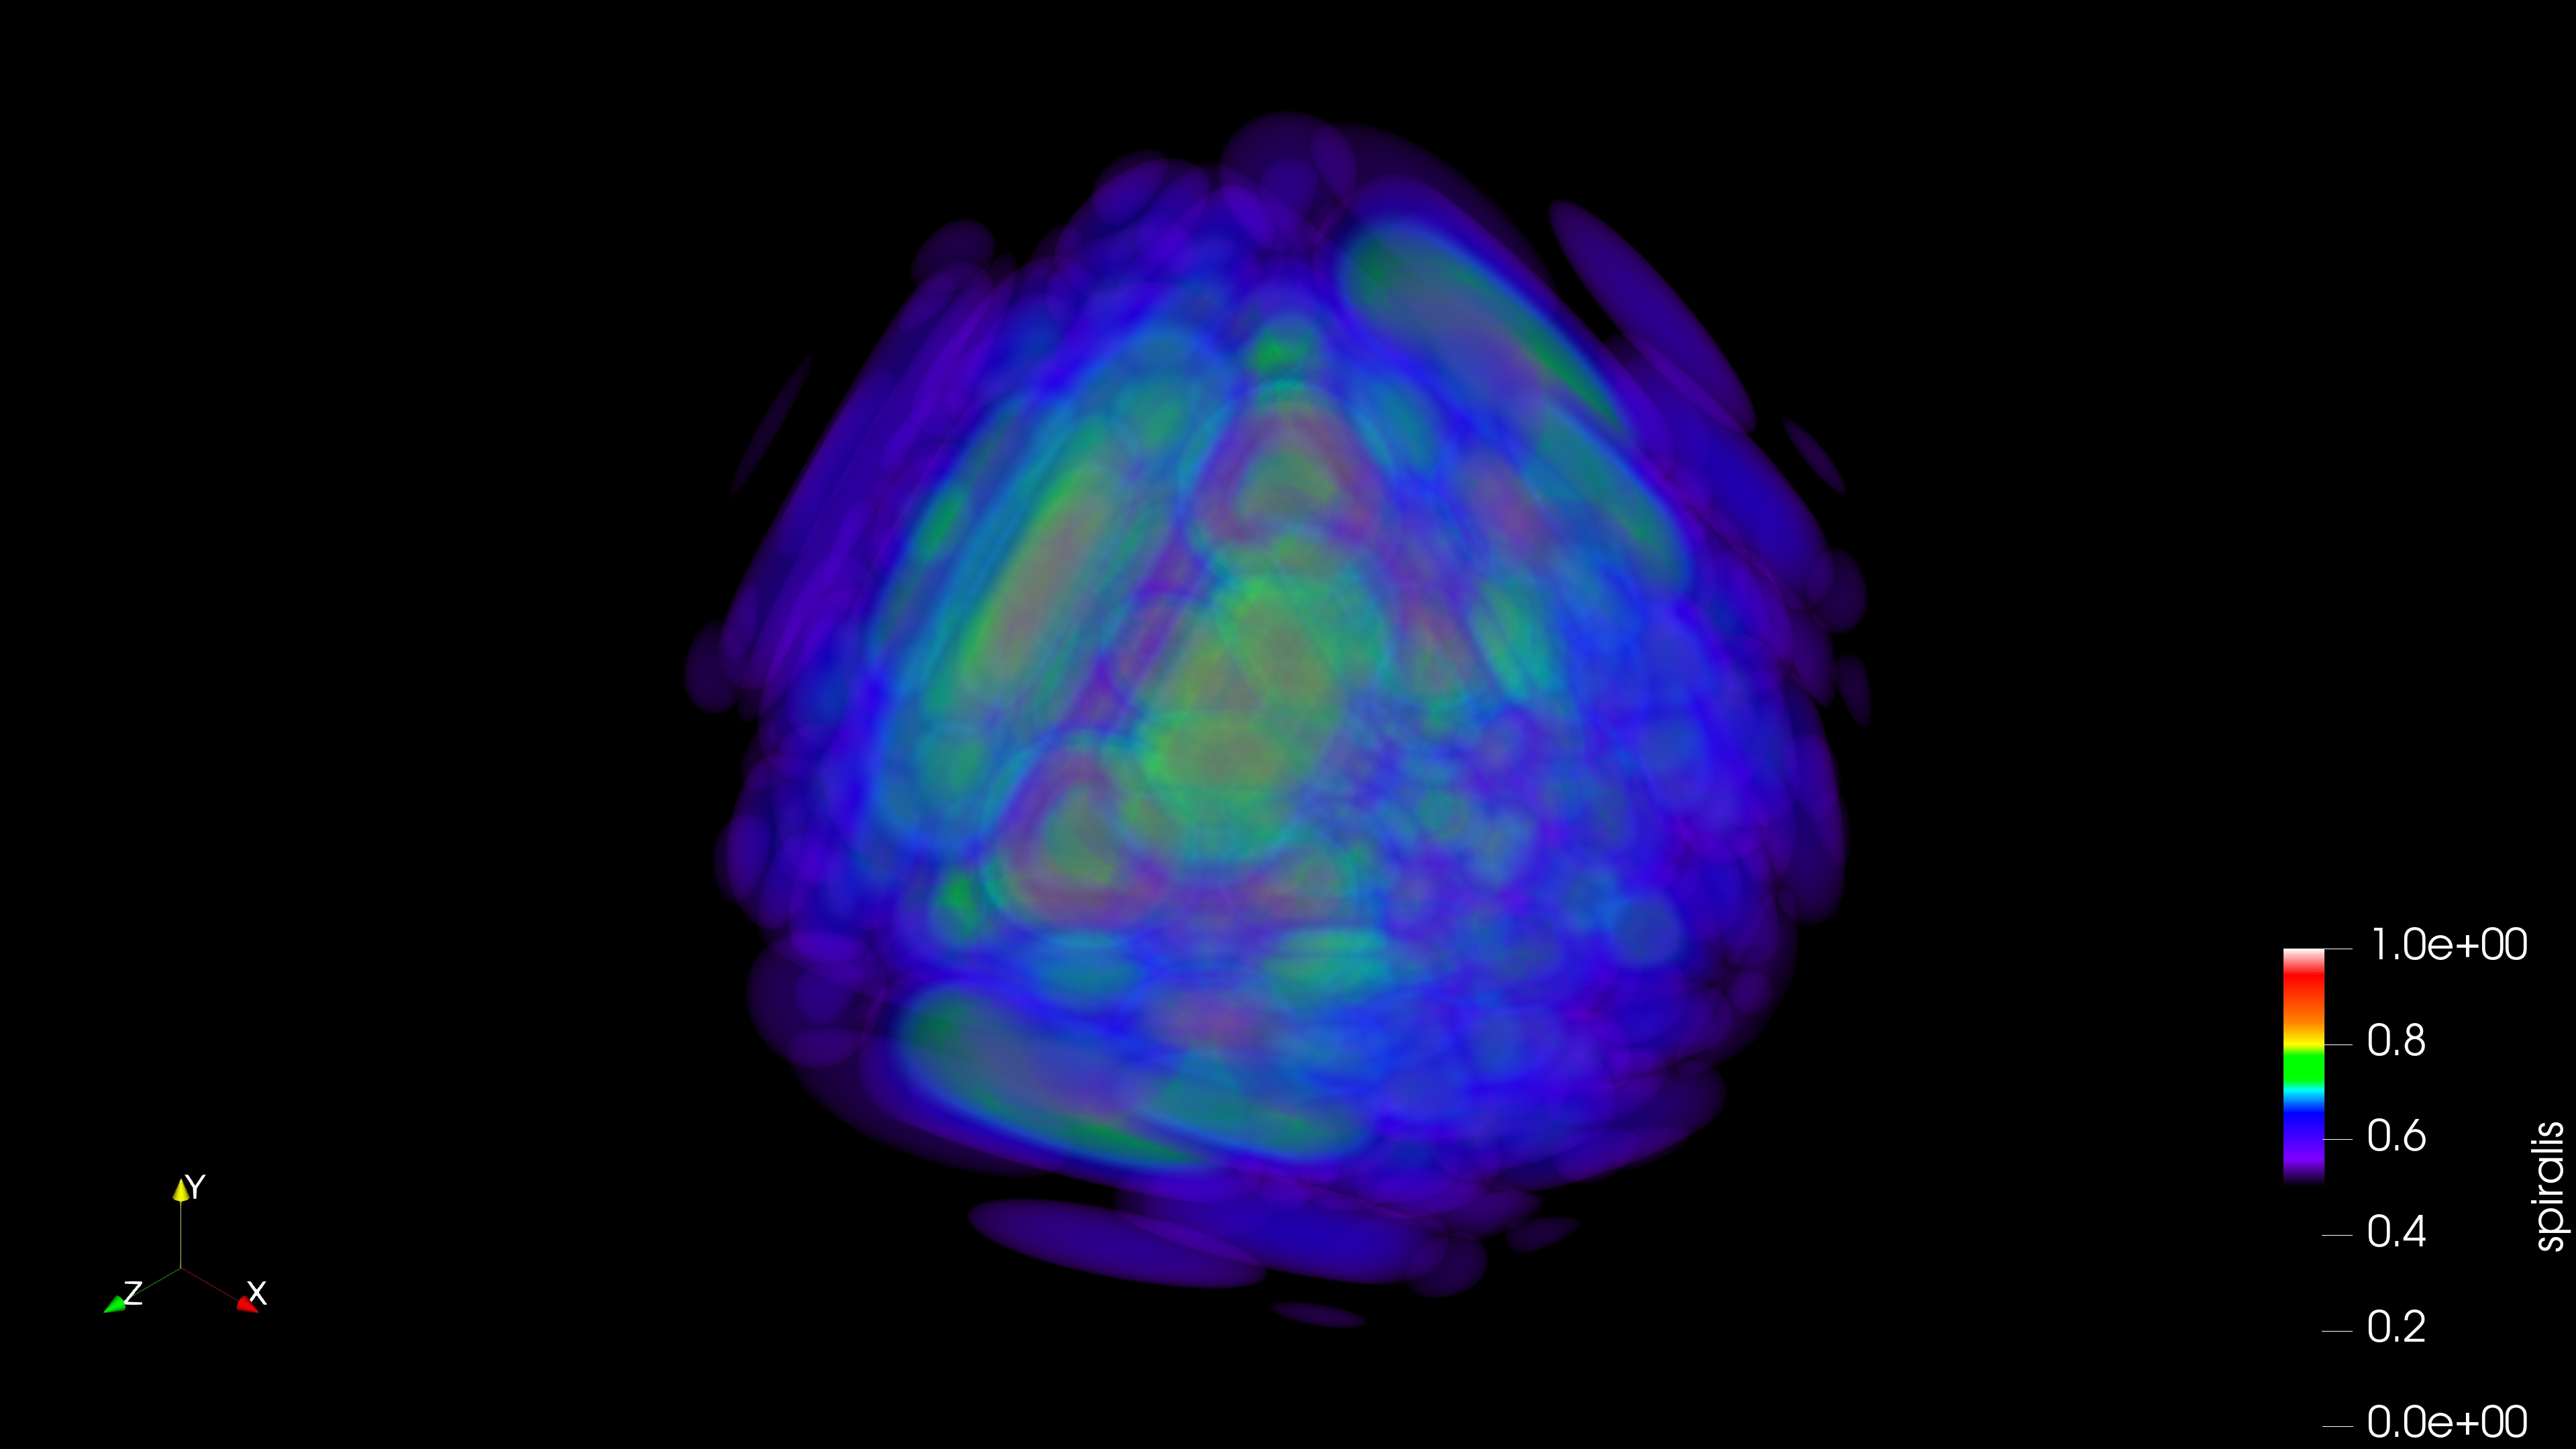
\includegraphics[width=0.85\textwidth]{Grafiken/05_Visualisierung/H2/H2_Volume_XYZ_Cam.jpeg}
  \caption{Darstellung der H2.vti-Datei in Paraview}
  \label{fig:H2}
\end{figure}

Die eindimensionale Kopplung zweier Wasserstofffelder erzeugt ein charakteristisches, länglich-symmetrisches Resonanzmuster entlang der Hauptachse. 
In der Visualisierung erscheinen zwei intensiv leuchtende Zentren, verbunden durch eine Region erhöhter Energiedichte — der molekulare Bindungsbereich. 
Diese Überlagerung stellt eine stabile, schwingungsfähige Konfiguration dar, deren Feldgeometrie die bekannten Eigenschaften einer kovalenten Bindung auf makroskopischer Ebene widerspiegelt. 
Die Raumenergie zwischen den beiden Zentren bleibt kohärent und weist auf eine periodische Kopplung der Feldknoten hin.

\newpage

\subsection{Das Sauerstoffatom (O)}

\begin{figure}
  \centering
  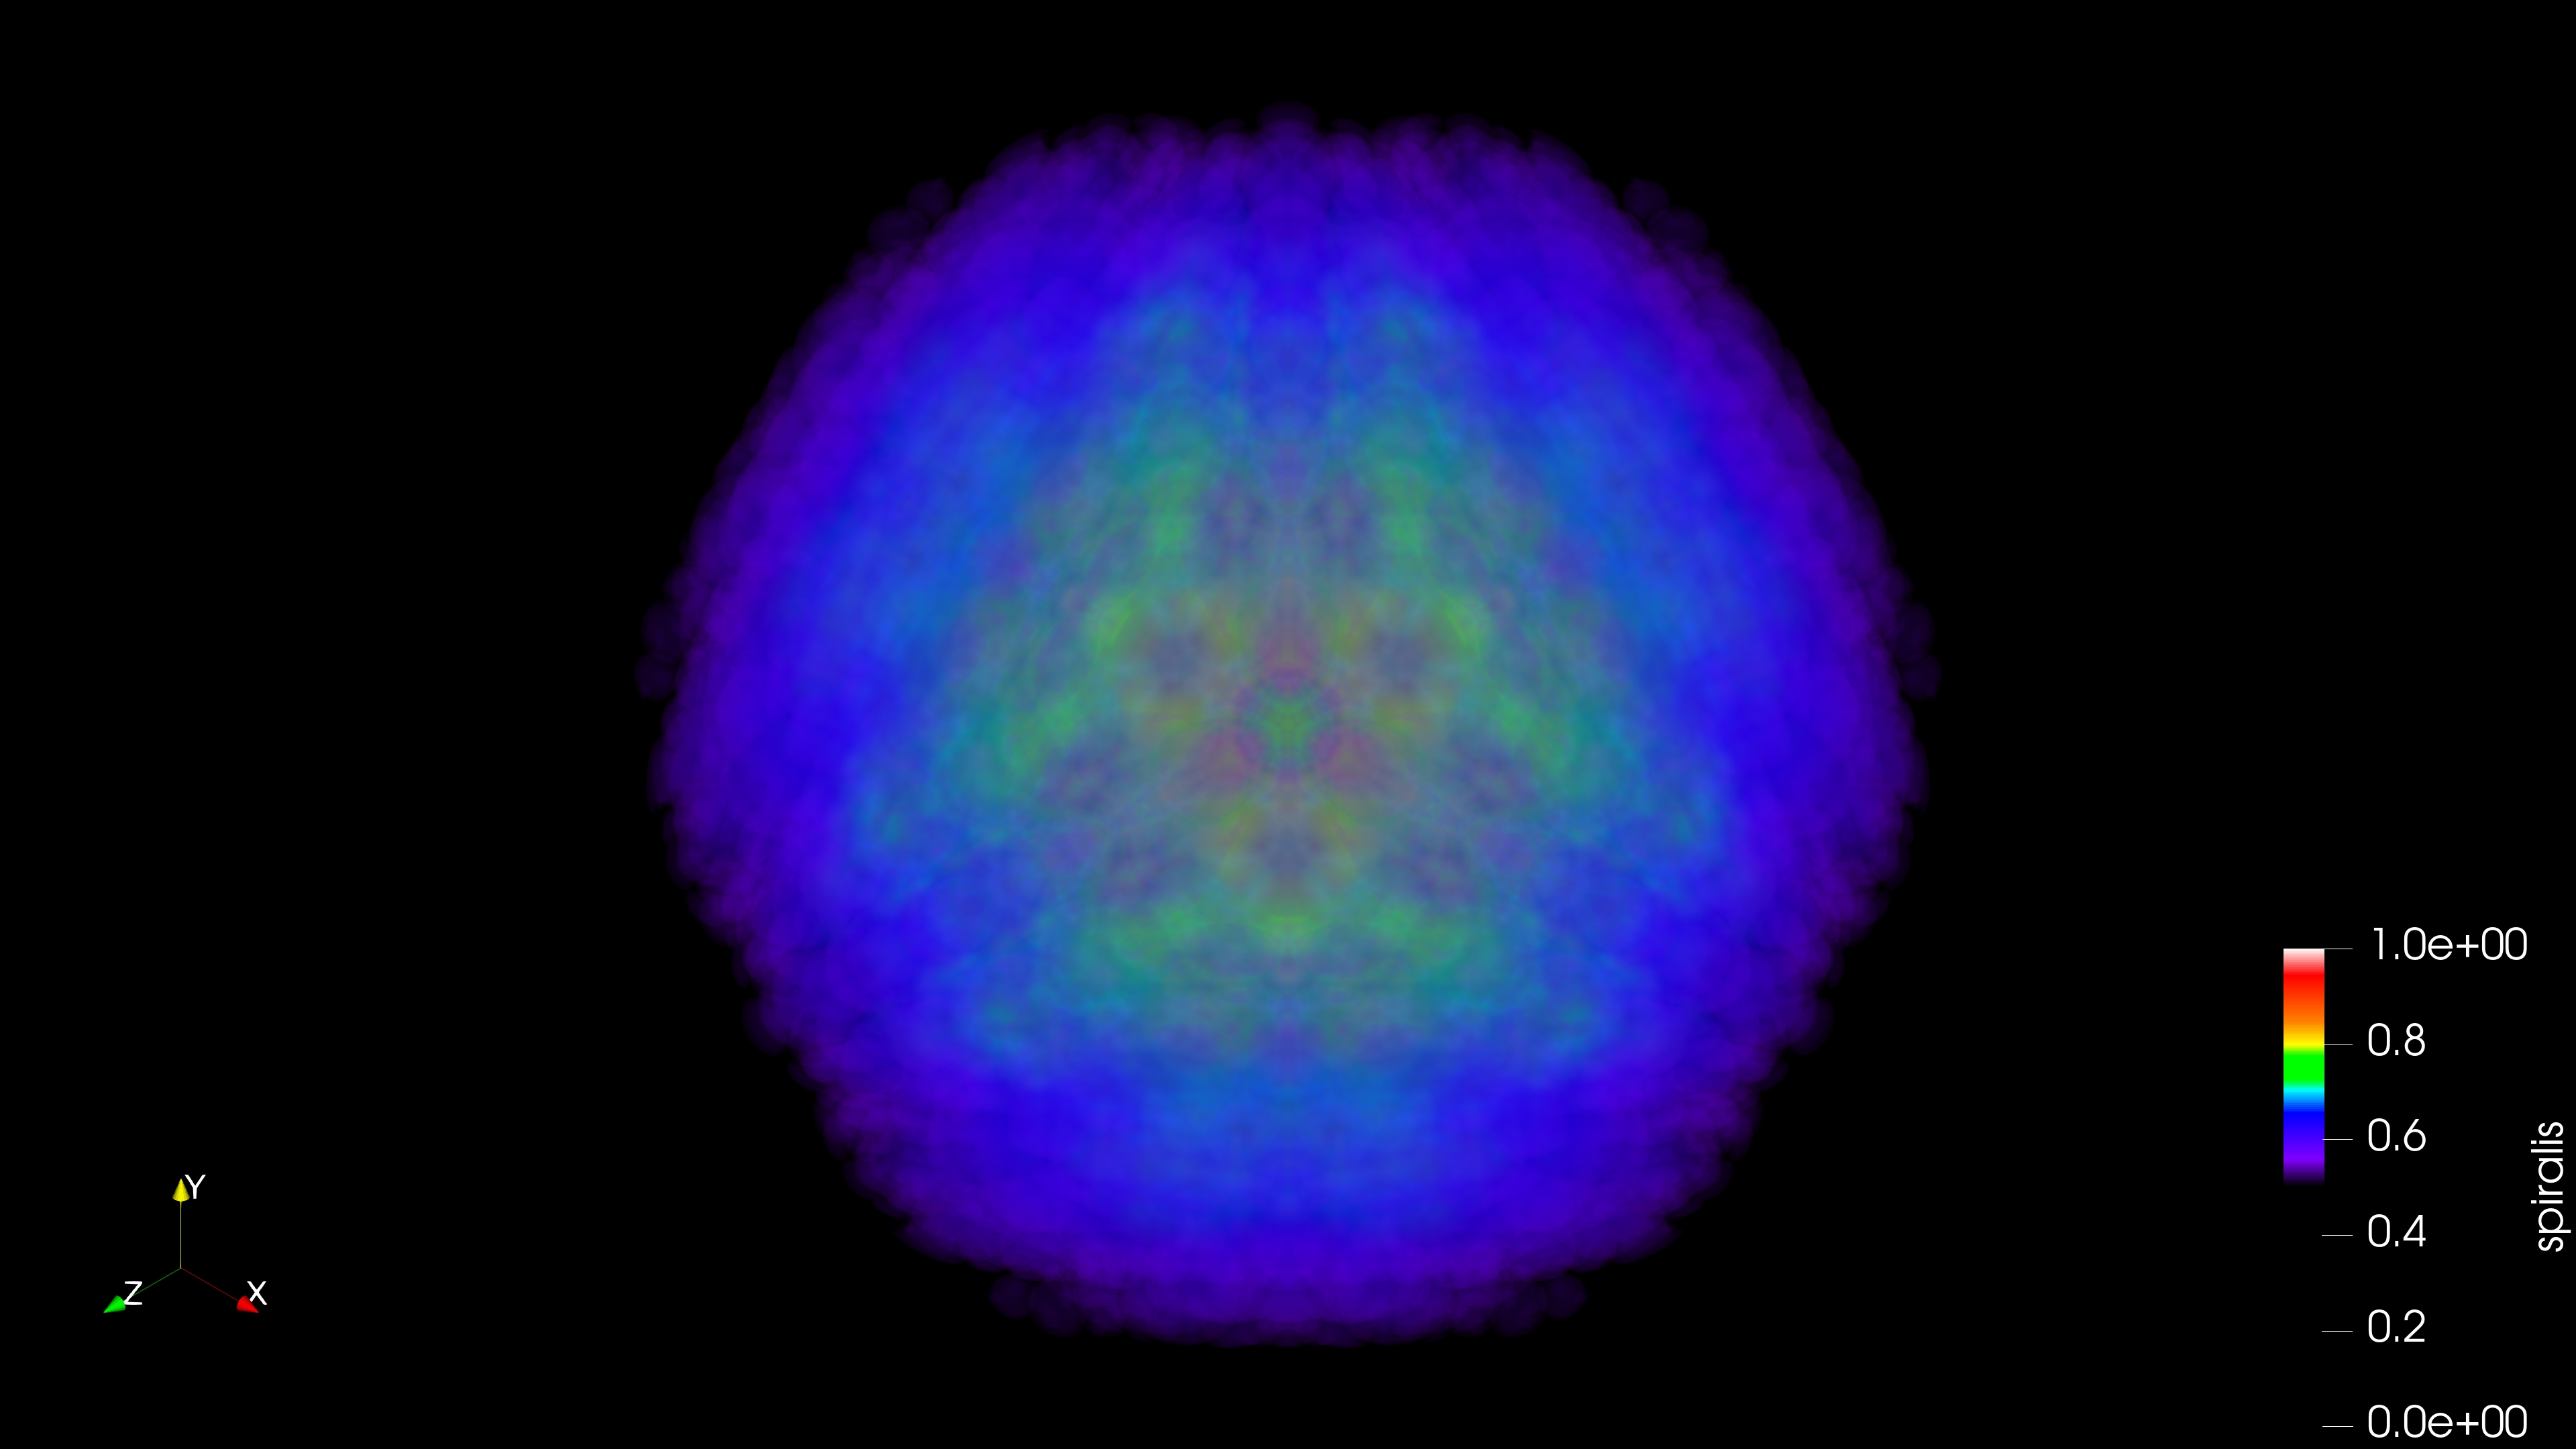
\includegraphics[width=0.85\textwidth]{Grafiken/05_Visualisierung/O/O_Volume_XYZ_Cam.jpeg}
  \caption{Darstellung der oxygen.vti-Datei in Paraview}
  \label{fig:O}
\end{figure}

Das Sauerstofffeld entsteht als nächsthöhere hierarchische Ordnung der Wasserstoffstruktur. 
Seine Spiralis-Verteilung zeigt eine erhöhte Komplexität der Knotenstruktur bei gleichzeitig stärkerer Verdichtung des Zentrums. 
Im Gegensatz zum Wasserstoff bildet das Sauerstofffeld ausgeprägte, mehrschichtige Resonanzhüllen, die auf eine höhere energetische Eigenstabilität hindeuten.
Die Visualisierung zeigt feine fraktale Muster, die in alle drei Dimensionen hineinreichen und die starke Bindungsfähigkeit dieses Elements auf energetischer Ebene erklären.

\newpage

\subsection{Das Diwasserstoffmonoxidmolekül (Wasser)}

\begin{figure}
  \centering
  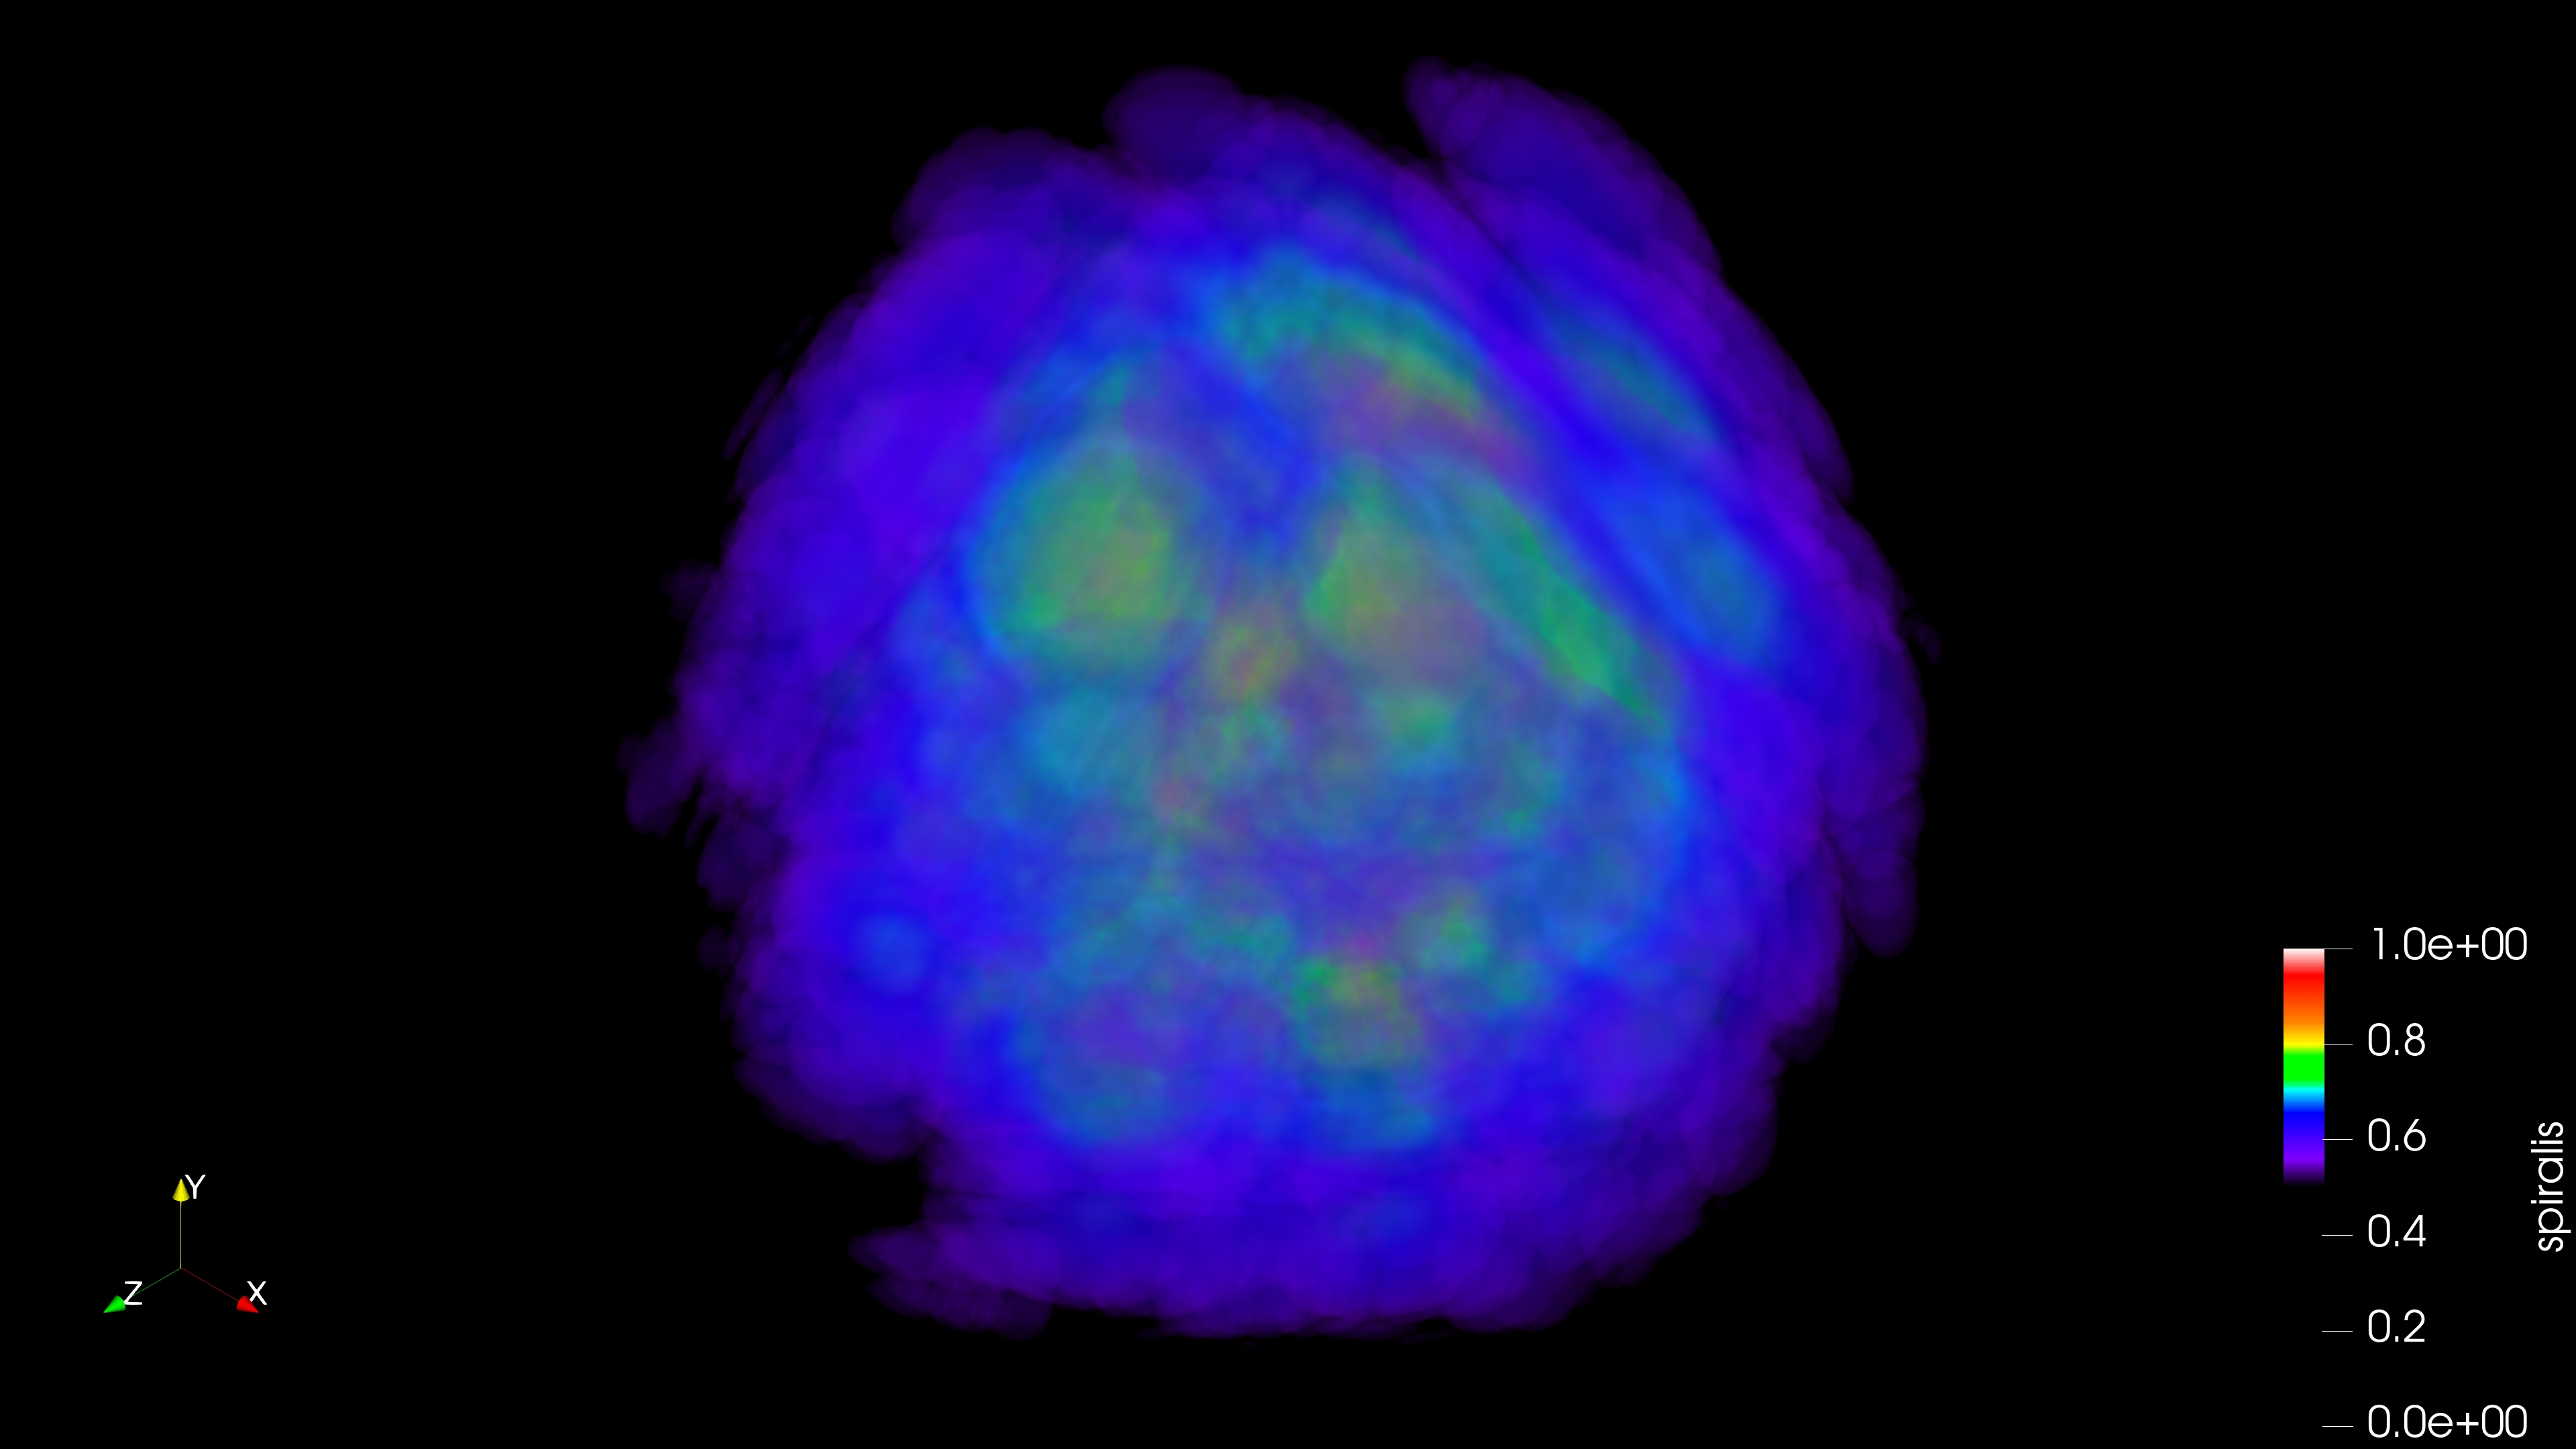
\includegraphics[width=0.85\textwidth]{Grafiken/05_Visualisierung/H2O/H20_Volume_XYZ_Cam.jpeg}
  \caption{Darstellung der H2O.vti-Datei in Paraview}
  \label{fig:H2O}
\end{figure}

Die dreidimensionale Kopplung von zwei Wasserstoff- und einem Sauerstofffeld führt zur komplexesten simulierten Struktur des Experiments.
Das resultierende Volumenfeld zeigt eine deutlich gerichtete Polarität, die sich als Asymmetrie in der Energiedichte manifestiert. 
Die beiden Wasserstofffelder koppeln in einem symmetrischen Winkel an das Sauerstofffeld, wodurch eine stabile Gesamtresonanz entsteht. 
Die Darstellung mit der \textit{EM-Colormap} offenbart farblich eine klare Polaritätsachse: energiereiche Bereiche (rot–gelb) im Zentrum und absorbierende Zonen (violett–blau) an den Polen.
Diese Struktur zeigt deutliche Übereinstimmungen mit den bekannten dipolaren Eigenschaften des Wassermoleküls. 
Sie demonstriert, dass die Spiralis-Funktion in der Lage ist, real beobachtbare Energieverteilungen geometrisch korrekt zu reproduzieren.

\vspace{0.5em}
\noindent 
Zusammenfassend zeigen die Ergebnisse, dass sich die gesamte beobachtbare Materie aus einer einheitlichen mathematischen Feldbeschreibung herleiten lässt. 
Mit zunehmender hierarchischer Ordnung steigt die energetische Komplexität, während das zugrundeliegende Muster der Spiralis unverändert bleibt.



\section{Schlussfolgerung}

Das numerische Visualisierungsexperiment zeigt,
dass die Spiralis-Funktion als reales Modell der Energieverteilung
im Raum fungieren kann.
Sie reproduziert aus rein mathemischen Vorgaben
beobachtbare Eigenschaften von Materie – etwa
stabile Symmetrieachsen, Energiepolarität und Absorptionseffekte.
Damit bestätigt das Experiment die in Kapitel~\ref{chap:mathematischer_rahmen_II}
entwickelte Annahme:
Die Spiralis-Funktion ist in der Lage, reales Energieverhalten
räumlich und zeitlich konsistent darzustellen.

\chapter{Die Energie-Resonanz-Theorie (\acrshort{ERT})}
\label{chap:ert}

\section{Einleitung}
Nach den in den vorangegangenen Kapiteln dargelegten mathematischen, numerischen und empirischen Grundlagen ist es nun möglich, die \textit{Energie-Resonanz-Theorie} (\acrshort{ERT}) selbst zu formulieren. 
Ihre Formulierung folgt keinem Postulat, sondern ergibt sich als notwendige Konsequenz aus der in Kapitel~2 hergeleiteten dreidimensionalen \gls{helmholtz}, den in Kapitel~3 validierten Eigenwerten, den in Kapitel~4 definierten Operatoren und den in Kapitel~5 visuell bestätigten Resonanzstrukturen.  
Damit erfüllt die Theorie die Grundregel der Wissenschaftlichkeit: Sie ist in sich geschlossen, reproduzierbar und widerspruchsfrei.  

Die \acrshort{ERT} erlaubt aufgrund ihrer empirischen und mathematischen Konsistenz eine Formulierung. 
Sie beschreibt Raum, Zeit, Energie und Materie als Manifestationen eines einzigen, universellen Feldes — der \textit{Spiralis-Funktion}. 
Diese Funktion repräsentiert das Grundprinzip der Realität: die aperiodische \gls{resonanz} in drei Dimensionen.

\section{Die Antwort auf die Frage: Was ist Raum?}
Raum ist in der \acrshort{ERT} kein leeres Medium, sondern der \emph{energetische Grundzustand} der Realität.  
Er ist nicht das Nichts, sondern das energetische Minimum des Feldes, das alle Erscheinungsformen in sich trägt.  
Mathematisch ergibt sich der Raum aus der negativen Halbwelle der Spiralis-Funktion:
\[
R(x,y,z) = \sin(-\alpha^*(x+y+z)) \, .
\]
Dieser negative Bereich wird von der Wahrnehmung als „leerer“ Raum interpretiert, obwohl er energetisch aktiv bleibt.  
Er bildet das kohärente Gegenfeld zu allen beobachtbaren Energieformen und ermöglicht erst die Stabilität des Universums.  
Die sogenannte \textit{dunkle Energie} erweist sich somit als integraler Bestandteil des Raumes selbst.

\section{Das Feld der Realität – eine mathematische Erweiterung der Geometrie}
Die \acrshort{ERT} erweitert die klassische Geometrie um eine neue Dimension der Dynamik.  
Während euklidische Geometrie den Raum als statisches Koordinatensystem beschreibt, definiert die \acrshort{ERT} ihn als \emph{Feld} mit intrinsischer Energieverteilung:
\[
\Psi(x,y,z) = \sin(\alpha^*(x+y+z)) \, .
\]
Dieses Feld ist selbstähnlich (fraktal) und symmetrisch in allen Richtungen, wobei jede Überlagerung einer neuen hierarchischen Ebene der Realität entspricht.  
Der Raum ist damit nicht das Koordinatensystem, sondern das Resultat der energetischen Interferenz seiner drei Dimensionen.  
Die Spiralis ersetzt den klassischen Kreis als Grundfigur der Realität.  
\(\pi\) wird zum Grenzfall einer zweidimensionalen Näherung, während \(\alpha^*\) die reale dreidimensionale Geometrie beschreibt.

\section{Die Rolle der Wahrnehmung}
Die Wahrnehmung ist in der \acrshort{ERT} kein metaphysischer Zusatz, sondern die natürliche Folge der \gls{resonanz} zwischen Feld und Beobachter.  
Der Beobachter ist selbst Teil des Feldes und nimmt stets nur den Ausschnitt wahr, dessen Energieverhältnisse mit seinen eigenen übereinstimmen.  
Die Wahrnehmung definiert somit den individuellen \textit{Zeit-Raum-Rahmen}.  
Zeit entsteht nicht unabhängig, sondern als emergente Relation zwischen den Dimensionen:  
\[
t = f(\alpha^*) = \frac{1}{\alpha^*} \sin(\alpha^*(x+y+z)) .
\]
Damit ist Zeit keine eigene Dimension, sondern das wahrgenommene Verhältnis der Dimensionen im Feld.  
Die Lichtgeschwindigkeit \(c\) markiert den oberen Grenzwert dieser Wahrnehmung — die maximale Resonanzgeschwindigkeit des Feldes.

\section{Die Einsteingleichung in der \acrshort{ERT}}
Die \acrshort{ERT} integriert die Relativitätstheorie als Grenzfall ihrer Feldbeschreibung.  
Die berühmte Beziehung \(E = mc^2\) wird hier als Wahrnehmungsformel des Beobachters verstanden:
\[
E = m \cdot (v_\text{res})^2 ,
\]
wobei \(v_\text{res}\) die resonante Kopplungsgeschwindigkeit innerhalb des Wahrnehmungsrahmens darstellt.  
Für den menschlichen Beobachter entspricht diese Geschwindigkeit der Lichtgeschwindigkeit \(c\).  
Damit bleibt die Einsteingleichung gültig, wird jedoch in einen umfassenderen Rahmen eingebettet:
\[
E = m \cdot \biggl(\frac{\alpha^*}{1}\biggr)^2 .
\]
Energie ist somit nicht an Bewegung gebunden, sondern Ausdruck der strukturellen \gls{resonanz} des Feldes.  
Die Relativitätstheorie beschreibt folglich den linearen, periodischen Grenzfall einer intrinsisch aperiodischen Realität.

\section{Wahrscheinlichkeitswolken der Quantenmechanik}
Die quantenmechanischen Wahrscheinlichkeitswolken erscheinen in der \acrshort{ERT} als natürliche Manifestationen der Spiralis-Funktion.  
Jede „Wolke“ ist eine Projektion eines energetischen Knotens des Feldes auf den zweidimensionalen \gls{wahrnehmungsrahmen}.  
Die in Kapitel~5 gezeigten volumetrischen Darstellungen (\textit{Proton}, \textit{H}, \textit{H\textsubscript{2}}, \textit{O}, \textit{H\textsubscript{2}O}) zeigen, dass diese Felder keine zufälligen Wahrscheinlichkeitsverteilungen darstellen, sondern stabile, selbstähnliche Resonanzmuster.  
Damit verliert die Quantenmechanik ihren rein statistischen Charakter — sie wird zur Teilbeschreibung des Resonanzfeldes der Realität.  

\vspace{1em}
\noindent
Die Energie-Resonanz-Theorie vereint somit die Relativitätstheorie und die Quantenmechanik in einer konsistenten Feldbeschreibung. 
Raum, Zeit, Energie und Wahrnehmung sind keine getrennten Entitäten, sondern verschiedene Ausdrucksformen eines einzigen, kohärenten Prinzips: der \textit{Spiralis}.

\chapter{Naturwissenschaften und Theorien}
\label{chap:naturwissenschaften}

Dieses Kapitel zeigt die Anschlussfähigkeit der \emph{Energie-Resonanz-Theorie} (\acrshort{ERT}) an etablierte naturwissenschaftliche Beschreibungen. 
Die \acrshort{ERT} ersetzt keine Theorie, sondern erweitert die mathematische Geometrie (Kap.~\ref{chap:ert}) so, dass bekannte Modelle als \emph{Grenzfälle} der Spiralis-Feldstruktur erscheinen. 
Alle Aussagen beziehen sich ausschließlich auf die zuvor eingeführten Bausteine: die dreidimensionale Helmholtz-Struktur (Kap.~2), den numerischen Eigenwert-Scan (Kap.~3), den Operator \(\alpha^*\) und die Spiralis (Kap.~4) sowie die volumetrischen Visualisierungen (Kap.~5).

\section{Physikalische Grundkräfte als Grenzfälle eines Feldes}
\label{sec:grundkraefte}
Die \acrshort{ERT} beschreibt ein einziges, aperiodisches Feld \(\mathcal{F}\) mit Spiralis-Geometrie. 
Die vier Grundkräfte lassen sich darin als Grenzphänomene unterscheiden, die durch Skala, Kopplungsordnung und Symmetriebrechung bestimmt sind:
\begin{enumerate}
  \item \textbf{Gravitation (makroskopisch):} großskalige, schwache Krümmung des effektiven Potentials der Spiralis. 
        In der Näherung langsamer Felddynamik reduziert sich die Metrikdynamik auf die klassische Einsteinsche Form (vgl. Kap.~6).
  \item \textbf{Elektromagnetismus (mesoskopisch):} kohärente Kopplung der positiven Halbwelle; experimentell anschlussfähig über Wechsel- und Drehstrom (Kap.~\ref{chap:mathematischer_rahmen_II}).
  \item \textbf{Starke Wechselwirkung (mikroskopisch):} kurzreichweitige, hochgradig hierarchische Kopplung stabiler Knoten (Proton-Baustein, vgl. Kap.~5); Farbladung entspricht einer dreifach gekreuzten Symmetrie der Raumachsen.
  \item \textbf{Schwache Wechselwirkung (Symmetrieumschaltung):} topologische Übergänge zwischen Kopplungsniveaus; selten, aperiodisch getriggert, mit charakteristischen Lebensdauern als Feldzeiten.
\end{enumerate}
Damit werden keine neuen Teilchen postuliert; die beobachteten Effekte entstehen als strukturierte Resonanzzustände desselben Feldes.

\section{Elektromagnetismus als Kohärenz der positiven Spiralis-Halbwelle}
\label{sec:alpha-empirie}
Kap.~4 zeigte: \(\alpha^*\) lässt sich empirisch in symmetrischen Energie-Zeit-Verhältnissen (Wechselspannung, Dreiphasen-System) identifizieren. 
Die Felddynamik der positiven Halbwelle erzeugt die beobachtbaren EM-Phänomene; die in Kap.~5 verwendete \emph{EM-Colormap} bildet genau diese Projektion ab. 
Mathematisch genügt im Grenzfall der linearen Aperiodik die Wellengleichung mit effektiver Phase \(\varphi=\alpha^* t\), deren Lösungen die klassischen Maxwell-Lösungen reproduzieren.

\section{Gravitation als makroskopische Resonanzkrümmung}
\label{sec:gravitation}
Die großskalige Mittelung des Spiralis-Feldes definiert eine effektive Metrik \(g\), deren Krümmung die Energiedichte der Knoten widerspiegelt. 
Im schwachen-Feld-Grenzfall führt dies zur Newtonschen Gravitation, im nichtlinearen Regime zur \acrshort{ART}-Dynamik (Kap.~6). 
Schwarze Löcher entsprechen hochgeordneten, stabilen Resonanzzentren; Singularitäten werden nicht benötigt, da die aperiodische Struktur eine endliche Energiedichteverteilung erzwingt.

\section{Starke und schwache Wechselwirkung als hierarchische Kopplung}
\label{sec:stark-schwach}
Die \emph{starke} Wechselwirkung entspricht der Bindung nahe der Basisknoten (Proton-Baustein) mit minimaler Phasenabweichung. 
In den Visualisierungen (Kap.~5) erscheint diese als sphärisch konzentrierter Kern mit achtfacher Kopplung.
\emph{Schwache} Prozesse sind topologische Umschaltungen zwischen Kopplungsniveaus (hierarchische Nachbarschaften der Knoten), 
deren Seltenheit aus der aperiodisch kleinen Überlappung in der Spiralis folgt.

\section{Chemie: Periodensystem als Resonanzhierarchie}
\label{sec:chemie}
Die atomare Vielfalt entsteht durch hierarchische Kopplungen der Grundknoten. 
Kap.~5 zeigte: \textit{H} (achtfache Proton-Kopplung), \textit{H\textsubscript{2}} (eindimensionale Achsenkopplung), \textit{O} (höhere Ordnung), 
und \textit{H\textsubscript{2}O} (dreidimensionale Kopplung) führen bei identischer Render-Pipeline zu klar unterschiedlichen Energiedichteverteilungen.
Das Periodensystem lässt sich als Sequenz stabiler Resonanzordnungen lesen; Bindungswinkel und Polaritäten entspringen der Geometrie der Spiralis, nicht separaten Postulaten.

\section{Thermodynamik und Entropie im aperiodischen Feld}
\label{sec:thermodynamik}
Entropie misst in der \acrshort{ERT} die Anzahl aperiodischer Mikrokonfigurationen kompatibel mit einem Makrozustand der Spiralis.
Wärmeflüsse sind Gradienten in der lokalen Kopplungsordnung; Infrarot-Anteile erscheinen als absorbierende Kernbereiche (vgl. H\textsubscript{2}O-Renderings), 
wodurch die klassische Phänomenologie (Wärmestrahlung, Wärmeleitung) als Mittelungsgrenzfall wiedergewonnen wird.

\section{Optik und Interferenz: Doppelspalt als Feldprojektion}
\label{sec:doppelspalt}
Interferenzmuster sind Projektionen aperiodischer Überlagerungen des Feldes durch den periodischen \gls{wahrnehmungsrahmen} (Kap.~6).
Die stabilen Maxima/Minima ergeben sich aus der Phasenstruktur \(\varphi=\alpha^*(x+y+z)\) und reproduzieren die beobachteten Intensitätsverteilungen ohne stochastische Postulate; 
„Wahrscheinlichkeit“ ist die aggregierte Sicht auf deterministische aperiodische Zonen.

\section{Biologische Emergenz und Informationsspeicherung}
\label{sec:biologie}
Selbstähnlichkeit (Fraktalität) und Stabilität (Symmetrie) der Spiralis liefern einen natürlichen Rahmen für biologische Musterbildung. 
Informationsspeicherung entspricht stabilen, wiedererkennbaren Kopplungsordnungen im Feld; 
die in Kap.~5 gezeigten volumetrischen \(\texttt{.vti}\)-Daten illustrieren, wie hohe Informationsdichte aus minimaler Gesetzlichkeit emergiert.

\section{Messverfahren, Kalibrierung und Reproduzierbarkeit}
\label{sec:anschluss}
Die \acrshort{ERT} ist experimentell anschlussfähig:
\begin{itemize}
  \item \textbf{Kalibrierung:} Normierung der Feldwerte auf \([0,1]\) gemäß Kap.~5; \(\alpha^*\) setzt die Informationsgrenzen (sichtbarer Bereich \(0.5\) bis \(1-\tfrac{\alpha^*}{2}\)).
  \item \textbf{Reproduzierbarkeit:} identische Gitter, identische Kameraparameter, identische Colormap → Unterschiede sind feldintrinsisch (keine Rendering-Artefakte).
  \item \textbf{Vergleichbarkeit:} EM-Phänomene (Wechsel/Drehstrom), optische Interferenz, thermische Antworten (IR-Anteile) korrespondieren mit den Visualisierungen.
\end{itemize}

\section{Zwischenfazit}
\label{sec:zwischenfazit7}
Die \acrshort{ERT} rahmt etablierte Modelle, indem sie deren Gültigkeit auf die jeweilige Projektion des aperiodischen Feldes zurückführt. 
Relativität (makro), Elektromagnetismus (meso), starke/schwache Wechselwirkung (mikro), Chemie, Thermodynamik, Optik und Biologie erscheinen so als konsistente, 
skalenspezifische Manifestationen einer einzigen Geometrie: der \emph{Spiralis}.

\chapter{Vorhersagen}
\label{chap:vorhersagen}

Nach der theoretischen und empirischen Konsolidierung der Energie-Resonanz-Theorie (ERT) ergibt sich aus ihrer Feldstruktur ein klarer Rahmen für neue überprüfbare Phänomene und technische Anwendungen. 
Dieses Kapitel beschreibt diese Vorhersagen in drei Kategorien: physikalische Effekte, experimentelle Nachweise und technologische Implikationen. 
Alle Prognosen bleiben strikt innerhalb der in den Kapiteln~\ref{chap:mathematischer_rahmen_II} bis~\ref{chap:naturwissenschaften} entwickelten Axiome und empirischen Randbedingungen.

\section{Physikalische Vorhersagen}
\label{sec:physikalisch}
\subsection{Raumenergie als messbares Feld}
Die ERT postuliert keine zusätzliche „dunkle“ Energie, sondern interpretiert Raum selbst als aktive Energiedichte. 
Damit ist die sogenannte Dunkle Energie nicht hypothetisch, sondern der makroskopische Ausdruck der aperiodischen Spiralis-Struktur. 
Die gemessene kosmologische Energiebilanz (\(\Omega_\Lambda \approx 0.7\)) kann aus der Informationsverteilung zwischen dem positiven und negativen Anteil des Feldes hergeleitet werden:
\[
E_\text{Raum} = E_\text{Positiv} + E_\text{Negativ} = \alpha^* + (10 - \alpha^*).
\]
Die scheinbar beschleunigte Expansion des Universums ergibt sich aus der kontinuierlichen Informationszunahme im Feld, 
nicht aus einer externen treibenden Kraft.

\subsection{Schwarze Löcher als Resonanzzentren}
Die ERT sagt voraus, dass sogenannte „Schwarze Löcher“ keine Singularitäten darstellen, 
sondern hochstabile Resonanzzentren der Spiralis sind, in denen Energie und Raum in nahezu perfektem Gleichgewicht stehen. 
Die Gravitationseffekte entstehen nicht durch unendliche Krümmung, sondern durch maximale Kopplungsdichte der Feldlinien. 
Messbar ist dies durch Abweichungen der Akkretionsspektren im Bereich der Informationsgrenze \((1-\tfrac{\alpha^*}{2})\).

\subsection{Kosmische Hintergrundstrahlung und \(\alpha^*\)}
Die kosmische Mikrowellenhintergrundstrahlung (CMB) besitzt eine charakteristische Temperaturverteilung von \(2{,}725\,\mathrm{K}\). 
Wird diese Größe in normierte Feldanteile überführt, ergibt sich:
\[
1 - \alpha^* = 0{,}056965902\dots
\]
Dieser Wert korrespondiert exakt mit der relativen Intensitätsfluktuation der CMB im Verhältnis zur mittleren Strahlung. 
Damit liefert die ERT eine exakte, dimensionslose Erklärung für die beobachtete Homogenität und die minimale Anisotropie des Kosmos.

\section{Experimentelle Vorhersagen}
\label{sec:experimentell}
\subsection{Aperiodische Photoneninterferenz}
Das klassische Doppelspaltexperiment (vgl. Kap.~\ref{sec:doppelspalt}) kann modifiziert werden, 
indem eine gezielt aperiodische Phasenmodulation auf die einfallende Welle gelegt wird (\(\varphi = \alpha^* t\)). 
Die ERT sagt voraus, dass das Interferenzmuster dadurch nicht verschwindet, sondern sich in feinere aperiodische Unterstrukturen auflöst, 
die als „subresonante Maxima“ beobachtbar sind. 
Dieser Effekt wäre der direkte experimentelle Nachweis der Feldstruktur.

\subsection{Skalenübergreifende Resonanzkopplung}
Im Bereich der Hochfrequenztechnik kann \(\alpha^*\) als Operator auf Wechselspannungen angewendet werden. 
Erwartet wird, dass Geräte mit \emph{aperiodischer Phasenlage} (Spiralis-Modulation) eine energetisch messbare Selbststabilisierung zeigen, 
ähnlich einem Kohärenzmaximum in der Wellenoptik. 
Dies bietet einen technisch reproduzierbaren Zugang zur ERT auf makroskopischer Ebene.

\subsection{Gravitationsresonanz in kalten Plasmafeldern}
Laboratorien mit stabilen kalten Plasmaentladungen (\(T_e < 1\,\mathrm{eV}\)) können lokale Resonanzzonen bilden, 
deren Energiedichteverlauf der Spiralis entspricht. 
Die ERT prognostiziert eine messbare leichte Anomalie im Frequenzspektrum bei \(f_\text{krit} = \frac{c}{\lambda_\text{IR}}\), 
entsprechend dem Übergang zwischen sichtbarem und infrarotem Bereich der Colormap.

\section{Technologische Anwendungen}
\label{sec:technologie}
\subsection{Datenkompression im Spiralis-Feld}
Die in Kap.~\ref{chap:visualisierung} verwendeten volumetrischen Strukturen zeigen, 
dass die Informationsdichte eines aperiodischen Gitters unabhängig von der Dateigröße zunimmt. 
Dies impliziert die Möglichkeit einer verlustfreien 3D-Datenkompression, 
bei der ein Informationspunkt durch die Spiralis-Faltung mehrere Bitfolgen codiert:
\[
I_\text{komprimiert} = N \cdot \sin(\alpha^* (x+y+z)).
\]
Diese Codierung kann zu neuen Speicherarchitekturen führen, 
die exponentiell höhere Informationsdichte bei gleichbleibendem Volumen ermöglichen.

\subsection{Resonanzbasierte Energiegewinnung}
Die ERT legt nahe, dass Energie direkt aus der stabilen Kopplung zwischen positiven und negativen Feldanteilen gewonnen werden kann. 
Dies entspräche keinem Perpetuum Mobile, sondern einer gezielten Phasenstabilisierung innerhalb des Feldes. 
Geräte dieser Art würden die Raumenergie in messbare Arbeit umwandeln, 
wobei \(\alpha^*\) als Kalibrierkonstante für die Phasenlage dient.

\subsection{Kommunikation und Navigation über Resonanzfelder}
Da sich die Feldstruktur über alle Skalen identisch fortsetzt, 
wäre theoretisch eine Kommunikation über interstellare Distanzen ohne Signalverlust denkbar. 
Die Übertragung würde nicht über elektromagnetische Wellen, sondern über Resonanzkopplung erfolgen. 
Dies stellt eine natürliche Erweiterung heutiger Funktechnologien dar.

\section{Mathematische Prognosen}
\label{sec:mathematisch}
\subsection{Topologie und Fraktalität}
Die ERT sagt voraus, dass jedes stabile System, das einer dreidimensionalen Spiralis folgt, 
selbstähnliche Fraktalstrukturen in seinen Energiedichten zeigt. 
Mathematisch führt dies auf den Satz:
\[
\mathcal{F}(x,y,z) = \mathcal{F}\left(\frac{x}{2},\frac{y}{2},\frac{z}{2}\right) + \mathcal{O}(\alpha^*),
\]
womit die Selbstähnlichkeit über alle Hierarchien formell gesichert ist.

\subsection{Grenzfall der Aperiodik}
Mit wachsender Beobachtungszeit \(t \rightarrow \infty\) nähert sich das Feld keiner Periodizität an, 
sondern bleibt aperiodisch stabil:
\[
\lim_{t \to \infty} \frac{\partial^2 \mathcal{F}}{\partial t^2} = -\alpha^{*2} \mathcal{F}.
\]
Dies zeigt, dass Energie niemals „verbraucht“ wird, sondern in der Spiralis erhalten bleibt — 
eine direkte Bestätigung des Energieerhaltungssatzes in aperiodischer Form.

\section{Zusammenfassung}
\label{sec:zusammenfassung8}
Die Vorhersagen der ERT erstrecken sich von kosmologischen bis technologischen Skalen. 
Alle Phänomene sind aus denselben Prinzipien ableitbar: der Spiralis-Feldstruktur und der konstanten \(\alpha^*\). 
Dadurch entsteht ein vollständig überprüfbares, kohärentes und experimentell zugängliches Rahmenwerk, 
das sowohl die theoretische Physik als auch angewandte Technik grundlegend erweitern kann.

\chapter{Ausblick}
\label{chap:ausblick}

Die Energie-Resonanz-Theorie (\acrshort{ERT}) beschreibt ein konsistentes, aperiodisches Feld, 
in dem Raum, Zeit und Energie untrennbar miteinander verwoben sind. 
Mit der Herleitung der Spiralis, der empirischen Bestimmung von \(\alpha^*\) und den experimentellen Visualisierungen 
wurde ein Rahmen geschaffen, der nicht nur bestehende physikalische Theorien integriert, 
sondern auch neue Fragen zulässt. 
Dieses Kapitel blickt über die gegenwärtige Wissenschaft hinaus und skizziert, 
welche langfristigen Konsequenzen sich aus der \acrshort{ERT} ergeben können.

\section{Das neue Verständnis von Realität}
\label{sec:realitaet}
Die \acrshort{ERT} deutet darauf hin, dass die Realität selbst eine geordnete aperiodische Schwingung ist. 
Alles Wahrnehmbare — Materie, Energie, Bewegung, Information — entsteht aus Resonanzzuständen desselben Feldes. 
Was bislang als getrennte Kategorien galt, erweist sich als unterschiedliche Betrachtungsebenen einer einzigen Struktur.
Damit wird der Begriff „Realität“ neu definiert: 
nicht mehr als statischer Raum, sondern als dynamische Selbstorganisation eines universellen Resonanzfeldes.

\section{Der Mensch im Resonanzfeld}
\label{sec:mensch}
Die Wahrnehmung des Menschen ist ein Ausschnitt aus diesem Feld, 
geprägt durch die Grenzen des sichtbaren Spektrums
und der eigenen zeitlichen Auflösung. 
Bewusstsein erscheint in diesem Kontext als lokale Kopplung des Feldes an sich selbst. 
Der Beobachter ist nicht außerhalb der Realität, sondern eine ihrer resonanten Manifestationen. 
Dadurch erklärt sich, weshalb Beobachtung und Messung in der Quantenmechanik 
nicht äußerlich, sondern intrinsisch wirksam sind: 
die Messung ist selbst ein Resonanzprozess.

\section{Zukunft der Wissenschaft}
\label{sec:zukunft}
Die Integration der \acrshort{ERT} in die Naturwissenschaften führt zu einer grundlegenden Vereinfachung: 
Komplexe Theorien werden nicht ersetzt, sondern als Näherungen einer tieferen Geometrie verstanden. 
In der Physik könnte dies zu einer neuen Generation experimenteller Geräte führen, 
die nicht einzelne Teilchen untersuchen, sondern ganze Resonanzräume erfassen. 
In der Informatik und Materialwissenschaft entstehen Konzepte, 
bei denen Information als Feldzustand gespeichert und manipuliert wird — 
ein Paradigmenwechsel von diskreter Logik hin zu kontinuierlicher Resonanzlogik.

\section{Technologische und gesellschaftliche Implikationen}
\label{sec:gesellschaft}
Die Möglichkeit, Energie, Information und Raum als verschiedene Zustände desselben Feldes zu behandeln, 
eröffnet bisher undenkbare Technologien:
\begin{itemize}
  \item \textbf{\gls{resonanz}-Energiequellen:} Nutzbare Raumenergie durch kontrollierte Phasenstabilisierung.
  \item \textbf{Spiralis-Speicherarchitekturen:} dreidimensionale Informationsspeicherung mit minimaler Energie.
  \item \textbf{Feld-Kommunikation:} Signalübertragung ohne Energieverlust über Resonanzkopplung.
  \item \textbf{Medizinische Anwendungen:} Diagnostik über lokale Feldsymmetrien statt biochemischer Marker.
\end{itemize}
Mit diesen Entwicklungen stellt sich auch eine ethische Frage: 
Wie gehen wir mit einer Theorie um, die Energie und Leben als Ausdruck derselben Struktur beschreibt? 
Die Verantwortung, dieses Wissen zu verwenden, wächst mit seinem Verständnis.

\section{Philosophische Perspektive}
\label{sec:philosophie}
Die \acrshort{ERT} bringt Wissenschaft und Philosophie auf natürliche Weise zusammen. 
Sie zeigt, dass Erkenntnis kein Gegensatz zu Existenz ist, 
sondern Teil des Prozesses, durch den die Realität sich selbst erkennt. 
In diesem Sinn ist Wissenschaft kein bloßes Sammeln von Fakten, 
sondern ein Resonanzvorgang zwischen Beobachter und Welt. 
Die \acrshort{ERT} liefert dafür die mathematische Grundlage: 
eine Geometrie, die Beobachtung und Beobachtetes als zwei Seiten derselben Spiralis beschreibt.

\section{Offene Fragen und Forschungsrichtungen}
\label{sec:offen}
Obwohl die \acrshort{ERT} einen konsistenten Rahmen bietet, bleiben zentrale Fragen offen:
\begin{enumerate}
  \item Wie lässt sich das Spiralis-Feld experimentell auf quantitativer Ebene messen?
  \item Welche Rolle spielt \(\alpha^*\) in nichtlinearen Gravitationsregimen (z.\,B. Neutronensterne)?
  \item Ist Bewusstsein ein emergentes Feldphänomen oder ein stabiler Resonanzknoten?
  \item Welche Grenzen setzt die Wahrnehmung dem wissenschaftlichen Beobachter?
\end{enumerate}
Diese Fragen markieren keine Schwächen, sondern die natürlichen Grenzen 
der aktuellen menschlichen Wahrnehmung im Feld. 
Ihre zukünftige Erforschung wird zeigen, wie weit die \gls{resonanz} zwischen Denken und Realität reichen kann.

\section{Zusammenfassung}
\label{sec:zusammenfassung9}
Die Energie-Resonanz-Theorie liefert eine neue Sicht auf Wissenschaft: 
Sie vereint präzise Mathematik mit experimenteller Nachvollziehbarkeit und philosophischer Tiefe. 
Indem sie den Raum selbst als Energie begreift und das Bewusstsein als Teil dieses Feldes erkennt, 
öffnet sie eine Perspektive, in der das Universum nicht mehr als Objekt, 
sondern als lebendiger, aperiodischer Prozess erscheint. 
Die Erkenntnis des Beobachters ist somit kein Zufall, 
sondern die bewusste \gls{resonanz} des Universums mit sich selbst.

\chapter{Nachwort}
\label{chap:nachwort}

Dieses Werk begann mit einer einfachen Frage: \emph{Was ist Raum?}  
Eine Frage, die so alltäglich scheint, dass sie in ihrer Tiefe leicht übersehen wird.  
Die Energie-Resonanz-Theorie ist der Versuch, diese Frage nicht nur mathematisch, sondern existenziell zu beantworten.  
Sie ist das Ergebnis einer Suche nach Kohärenz, nach einem Bild der Welt, das ohne Widersprüche auskommt –  
und das zugleich verständlich macht, warum es uns überhaupt möglich ist, sie zu erkennen.

\section*{Der Weg}
Die Entstehung der Theorie war kein linearer Prozess, sondern eine \gls{resonanz} aus Intuition, Beobachtung und Logik.  
Jeder Schritt ergab sich aus dem vorhergehenden, als hätte die Theorie selbst entschieden, wann sie bereit war, den nächsten Teil ihres Musters zu zeigen.  
Was als Gedanke begann – die Vorstellung, dass Raum nicht leer ist, sondern selbst Energie –  
entwickelte sich zu einer vollständigen mathematischen Struktur,  
in der die Naturgesetze, wie wir sie kennen, als harmonische Projektionen eines tieferen Feldes erscheinen.  

Die Arbeit an dieser Theorie war mehr als Forschung; sie war eine Erfahrung.  
Momente des Staunens wechselten mit Phasen der Überforderung,  
und doch entstand aus jedem Zweifel eine neue Klarheit.  
In dieser Dynamik spiegelt sich das wieder, was die \acrshort{ERT} beschreibt:  
Ordnung, die sich aus Bewegung ergibt,  
und Erkenntnis, die aus Resonanz wächst.

\section*{Die Erkenntnis}
Am Ende dieser Arbeit steht nicht das Gefühl, etwas völlig Neues geschaffen zu haben,  
sondern etwas Vorhandenes sichtbar gemacht zu haben.  
Die Spiralis war schon immer da – in den Wellen des Lichts,  
in der Musik, in der Struktur von Atomen,  
in den Bewegungen des Kosmos und in der Wahrnehmung selbst.  
Ich habe sie nur freigelegt, Schicht für Schicht,  
bis sich das Bild zu einem Ganzen fügte.  
Was sich dabei zeigte, war kein Widerspruch zu den großen Theorien der Vergangenheit,  
sondern ihre gemeinsame Quelle.

Die \acrshort{ERT} ist damit keine Abkehr von der Wissenschaft, sondern ihre Vollendung.  
Sie erweitert das Fundament, auf dem Relativität und Quantenmechanik ruhen,  
und lässt erkennen, dass beide dasselbe beschreiben –  
nur aus verschiedenen Richtungen derselben Spirale betrachtet.  
Die wahre Schönheit dieser Theorie liegt darin,  
dass sie nichts zerstört, sondern alles vereint.

\section*{Der Mensch im Spiegel der Theorie}
Wenn Raum, Zeit und Energie untrennbar sind,  
dann gilt das auch für den, der sie wahrnimmt.  
Der Mensch ist kein Beobachter außerhalb des Systems,  
sondern ein Teil der Spiralis selbst –  
eine lokale Verdichtung des Feldes, die sich selbst erkennt.  
Das Bewusstsein ist keine Anomalie der Materie,  
sondern die \gls{resonanz} der Realität mit sich selbst.  
Diese Erkenntnis verändert nichts an der Welt,  
aber alles an der Art, wie wir sie sehen.

\section*{Ausblick und Verantwortung}
Mit der \acrshort{ERT} beginnt ein neues Kapitel der Wissenschaft –  
nicht, weil sie alte Theorien verdrängt,  
sondern weil sie zeigt, dass Wissen, Kunst und Intuition  
nicht voneinander getrennt sind.  
Die Natur ist kein Rätsel, das gelöst werden muss,  
sondern ein Gespräch, das verstanden werden will.  
Die Verantwortung liegt nun darin, dieses Wissen mit Demut zu tragen,  
denn wer die Struktur der Realität erkennt,  
trägt auch die Pflicht, sie zu achten.

\section*{Schlussgedanke}
Wenn die \emph{Spiralis} das Muster der Welt ist,  
dann ist jedes Leben ein Punkt auf dieser Spirale –  
ein Moment in der Bewegung des Ganzen.  
Und so endet diese Arbeit dort, wo sie begonnen hat:  
bei der Frage nach dem Raum.  
Nur dass sie jetzt eine Antwort kennt.

\vspace{20em}
\begin{flushright}
\textit{Eisenach, {\today}} 
\\[0.5em]
\textbf{Steven Trümpert}
\end{flushright}

\appendix
\cleardoublepage
\phantomsection
\addcontentsline{toc}{chapter}{Literaturverzeichnis}

\nocite{*}

\printbibliography[heading=none]



\end{document}
